%FIX sign post
%MAYBE existing literature pedometer vs strength 
%FIX every stage of the document mention the research question
%FIX FOCUS 
%FIX user table
%FIX explain scales
%FIX survey results/interview results separately
%FIX requirements moscow
%FIX conclusion longer what motivation results interview conditions
%user stories depend on 


% REMEMBER: You must not plagiarise anything in your report. Be extremely careful.

\documentclass{l4proj}

% put any additional packages here

\begin{document}

%==============================================================================
%% METADATA
\title{Stat Buff: Collaborative Strength Exercise Tracker}
\author{Eerik Saksi}
\date{April 7th 2021}

\maketitle

%==============================================================================
%% ABSTRACT

\begin{abstract}
    \vskip 0.5em

I created Stat Buff, which is a crossover between a strength exercise tracker and a collaborative multiplayer RPG. There has been a lot of promising research into pure collaborative activity trackers, where a user's contribution only influences their own team. I wanted to investigate whether a hybrid tracker would outperform personal trackers and collaborative trackers. In my hybrid tracker, users have an individualistic as well as a shared goal. This caters to users who like to train with others as well as those who want to train alone. I also wanted to investigate whether the success of existing collaborative trackers would generalize in to strength training gamified as an RPG. Most existing research on collaborative trackers focus on pedometers, and there has been no research on whether it generalizes to other forms of exercise, such as strength training. In addition, most apps reward exercise by simply increasing the user's group's score. I tried to make progression more interesting and satisfying by applying existing techniques from RPG games, which no other collaborative activity tracker has done before. When users start using the app, they are given a virtual character. This character's strength and appearance are proportional to the user's real life strength, which motivates the user to increase it. They can also join a team with other virtual characters. Teams are assigned a monster enemy which they are tasked with killing. Killing this monster will progress your entire team forward, and give you a new enemy to fight. Individual characters in teams can deal damage to the monster by completing a training session. This means that users can both develop their individual character through becoming stronger, as well as their team through working out. In my evaluation, I primarily investigated the interest in the personal and shared goal. From this, I could deduce whether there were users who would've dropped out if there wasn't a secondary goal which they could pursue. Although the mean ratings were roughly the same, the sentiment towards shared goals was much more spread out, which made individual goals a good stable fallback. 

\end{abstract}


\newpage
\chapter*{Acknowledgements}
I want like to thank my supervisor, Dr. Alistair Morrison for all his help and support, especially with regards to the evaluation of the app. Without his help, my evaluation wouldn't have had a clear goal and my interviews, surveys, and data analysis would've been conducted poorly. I would like to thank my friend Jaakko, with whom I brainstormed many ideas for the project and conducted a pilot study with. Finally, I would like to thank all my participants for using my app, especially those who took time out of their day to conduct an interview.

%==============================================================================

% EDUCATION REUSE CONSENT FORM
% If you consent to your project being shown to future students for educational purposes
% then insert your name and the date below to  sign the education use form that appears in the front of the document. 
% You must explicitly give consent if you wish to do so.
% If you sign, your project may be included in the Hall of Fame if it scores particularly highly.
\def\consentname {Eerik Saksi} % your full name
\def\consentdate {31 March 2021} % the date you agree

\educationalconsent


%==============================================================================
\tableofcontents

%==============================================================================
%% Notes on formatting
%==============================================================================
% The first page, abstract and table of contents are numbered using Roman numerals and are not
% included in the page count. 
%
% From now on pages are numbered
% using Arabic numerals. Therefore, immediately after the first call to \chapter we need the call
% \pagenumbering{arabic} and this should be called once only in the document. 
%
% Do not alter the bibliography style.
%
% The first Chapter should then be on page 1. You are allowed 40 pages for a 40 credit project and 30 pages for a 
% 20 credit report. This includes everything numbered in Arabic numerals (excluding front matter) up
% to but excluding the appendices and bibliography.
%
% You must not alter text size (it is currently 10pt) or alter margins or spacing.
%
%
%==================================================================================================================================
%
% IMPORTANT
% The chapter headings here are **suggestions**. You don't have to follow this model if
% it doesn't fit your project. Every project should have an introduction and conclusion,
% however. 
%
%==================================================================================================================================

%setting the scene
\chapter{Introduction}

\section{Motivation}
%FIX step counts, same mechanisms apply 

Activity trackers are tools which are used to plan and log exercise. They are primarily marketed as motivators to exercise, and often contain additional features such as social feeds and competitions. Collaborative activity trackers are a variation of activity trackers with built-in collaboration. When using these trackers, your exercise helps your teammates in some way. If implemented well, this creates additional motivation as users want to help their team progress or feel an obligation to help. There is some existing research into collaborative activity trackers, which generally perform better than competitive or individual tracking. Existing collaborative trackers all measure step counts and movement which can be done automatically. 

This projects investigates the effectiveness of a hybrid model: a combination of an individual tracker and a collaborative tracker. This means that there is both a personal goal for each user, as well as a team goal which they can contribute to. There are no other collaborative activity trackers which have a separate personal goal, and vice versa. I wanted to research whether this would be superior to a regular tracker with just one goal. The advantage of my app is that participants who do not care about the personal goal may still be interested in the team goal, and vice versa. The other goal can serve as a fallback, which may maintain a user who would've otherwise quit. There may also be users who are motivated by the personal and shared goal, motivating them more than other apps could. The biggest cost of my hybrid model is that users potentially have to understand twice as much in order to participate. 

My app implements both the personal and shared goal through an RPG model. RPGs (Role Playing Games) refer to games such as World of Warcraft which are set in fictional medieval worlds with supernatural elements such as monsters and magic. In these games, characters progression happens through skill development which requires laborious repetitive tasks, often referred to as "grinding". I decided to gamify exercise with an RPG model, as training is also built around doing laborious repetitive training exercises. RPGs also served as a good example of hybrid goal implementation: many online RPGs such as World of Warcraft let you develop your character, but also participate in group based challenges.


%MAYBE
%In order to ensure that my collaborative features were motivating, I had to apply techniques from various theories:
%
%Self-determination theory: One of the three mini-theories is that social relatedness induces motivation. 
%
%Social comparison theory: This theory argues that people change behavior based on how they are perceived by others. 
%
%Social support theory: This theory argues that positive social encounters are motivating.

\section{Aim}
The primary goal of my project will be to investigate the effectiveness of an activity tracker which has both personal and shared goals. In my evaluations I will seek out whether creating more goal diversity prevented drop-offs as I catered to more users, or increased them due to the additional complexity. As my app has other novel features compared to existing collaborative activity trackers, namely strength tracking and RPG features, I also wanted to investigate how the findings of other collaborative activity trackers generalized to my app. These were my two primary areas I wanted to address:
\begin{itemize}
  \item Does an activity tracker with both a personal and shared goal outperform trackers with single goals?
  \item Is the additional complexity of two goals worth the possible motivation increase?
\end{itemize}
  


\pagenumbering{arabic} 


%==================================================================================================================================
\chapter{Background}

\section{Background Literature}

\subsection{Collaborative Activity Trackers}
There is a lot of existing research into the effectiveness of collaborative activity trackers. Most of the research focuses on increasing step counts with pedometers. This differs slightly from my strength tracker, as walking is done in everyday life and can be automatically tracked, whilst strength training is usually deliberate and manual tracked. Strength training also has a higher barrier of entry: it often requires access to equipment, and understanding of exercise form and the muscle groups they train. My primary focus was to identify whether or not there was a collaborative activity tracker which also had a personal goal.

``Pass the Ball'' was an app which was developed in order to evaluate the effectiveness of enforced turn taking for encouraging exercise \citep{Pass_the_ball}. With the hybrid model, your own step count was the most important, but the other person had a small impact. In the second version of the app, users in groups had a single ball which gave the owner the ability to score points for the team through exercise, which could be passed to other users. Users who received the ball often felt that they had a small window of opportunity to score points before someone else wanted the ball. For example, one participant said: ``I turned to my group and I was like 'we’re walking fast today! We have an hour to get as many steps in as we can!'''. The exclusivity also led to some issues. Users who stole the ball from other teammates (incurring a penalty) would get into fights with other members. One user sent the message ``'Sorry, Just looked at my phone. I would have passed!'' after their ball was stolen. Although the app seemed to make some group members competitive and more passionate about exercise, there were some drawbacks to their implementation ``such as obligation, conflict, and privacy concerns''.

\citet{HealthyTogether} didn't just investigate the effectiveness of collaborative features, but also competitive ones, and combinations of the two. In the competitive model, step counts were scored relative to your opponent. In the collaborative model, you and your teammate contributed equally to your shared total points. Interestingly, the control group which exercised alone performed better than the group which competed amongst themselves. The collaborative model performed the best: ``Amongst the group settings cooperation (21\% increase) outperformed competition (8\% increase)''. This study supports collaborative activity trackers.

\citet{ChickClique} developed an app called ``Chick Clique'' which had a lot of the same design principles. They had assigned 5 different skill levels for users based on their step count, as well as a ``team average'' which girls collaborated together to improve on. My app also had 5 different characters and titles you got based on your strength, as well as progression based on average performance of each member. Chick Clique also included other health features such as tips for healthy eating. Despite the participants having a pedometer, food tips, and gamified progress ``group performance was rated by the girls as being the most powerful method of changing behavior.'' 

\citet{Fish'n'Steps} created a site called ``Fish'n'Steps''. The participants were given a virtual fishbowl, where the number of fish, their mood and their growth were influenced by the number of steps that they took. There was a version of the game which served as the control group where participants were given their own fishbowl, and thus did not collaborate or compete. The fishbowl which contained other fish was used to study the impact of collaboration/competition. The step counts of each user influenced the shared fishbowl: ``each 'insufficient' day for any team member resulted in the tanks water getting darker, as well as the gradual removal of the fish-tank’s decorations''. There was also out-group competition through leaderboards for the best performing teams. Much like my app, this site employed visual rewards. You got better looking characters as you got stronger, whilst this site grew your fish with more steps. I implemented shared visual rewards: you got to see the enemy update and it's health reduce as your team worked out, whilst this site varied the state of your fishbowl. This site also implemented anonymous teams, and also found that ``anonymous team cooperation did not produce significant results''.  The game led to good behavioural changes, but participants lost interest ``Although the initial fascination with the game subsided after the first couple of weeks, it nonetheless generated sustainable change in behavior and made continuing the game unnecessary.''

\citet{Shakra} estimated the activity of participants through their cell signals. This study was mostly focused on using neural networks to estimate activity. The estimated activity levels were shared with friends. The app performed well even without the social features: ``participants described how they would enjoy checking how much walking and running activity they did during the day.'' There wasn't much collaboration amongst teams, which instead competed. Competition seemed to be effective as users ``also enjoyed competing amongst themselves''. This is interesting, as users did not like competition in the aforementioned app Healthy Together. 

\citet{Stickers} developed ``Stickers for Steps'' an Android sticker collecting app. Stickers are collected through reaching step count targets. Users could receive duplicate stickers, which motivated users to trade stickers. Users could only trade them through Bluetooth, which encouraged users to meet face to face. This resembled the real experience: ``part of the joy of the sticker collecting experience is in meeting with others to exchange the inevitable duplicates that will accrue from the random sticker acquisitions''. This app brought users together as 27/31 of users who had partners traded at least once. Sticker swapping often served as an icebreaker: ``Conversations during and after sticker exchanges were reported to have been quite general, discussing the app itself as well as typical day-to-day chitchat''.

In order to make the most out of my collaborative feature, I had to understand how users are motivated by peers. Self-determination theory argues that an individual's experience of autonomy, competence, and social relatedness induce the most motivation \citep{self_determination_theory}. \citet{social_comparison_theory} argues that people change behaviour based on how they are viewed by others. Social support theory argues that positive social encounters encourage behaviour change \citep{social_support_theory}. 

\subsection{Top personal activity trackers}
 There are far more personal trackers than collaborative ones, so I tried to find studies which analyzed many at once. There have been studies looking at the behavioural change techniques used by these top apps as a whole. \citet{AppsOfSteel} scored 127 top exercise apps based on the presence or absence of various behavioural categories techniques. In terms of social features, the average exercise app only contained 2.67\% of all social behavioural change techniques.  

 \citet{weight_loss} analyzed 204 weight loss related apps. They also found that few apps implemented social support. Based on the poor use of social techniques in the top apps, it seems that there aren't apps which both implement collaborative and personal goals. 

 %MAYBE elaborate more

\section{Commercial Products}
I analyzed existing strength exercise trackers and existing RPG games in order to better understand the two categories I am combining. There are 5 rows for each app I am analyzing. My app is the first one, Stat Buff. I created 12 columns for features present in other apps, as well as my own. Green denotes presence of this feature, yellow denotes partial presence, and red denotes absence of this feature from this tracker.

\subsection{Activity Trackers}
\begin{figure}[H]
    \centering
    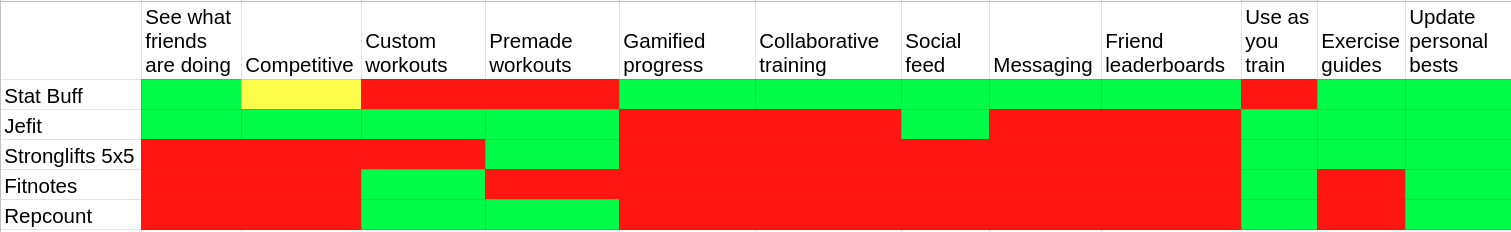
\includegraphics[width=1.0\linewidth]{exercise_comparisons.png}    
    \caption{Presence and absence of features in popular exercise apps}
    \label{fig:exercises} 
\end{figure}

You might notice that my app is the only one which lacks ``custom workouts'', ``premade workouts'' and ``use as you train''. I did not have time to make a full activity tracker. Users could only input their personal bests for specific exercises, and how long and intense their exercise was. In Figure \ref{fig:jefit} you can see Jefit's more nuanced workout tracking features which my app lacks:
\begin{figure}[H]
    \centering
    \begin{subfigure}{0.3\textwidth}
        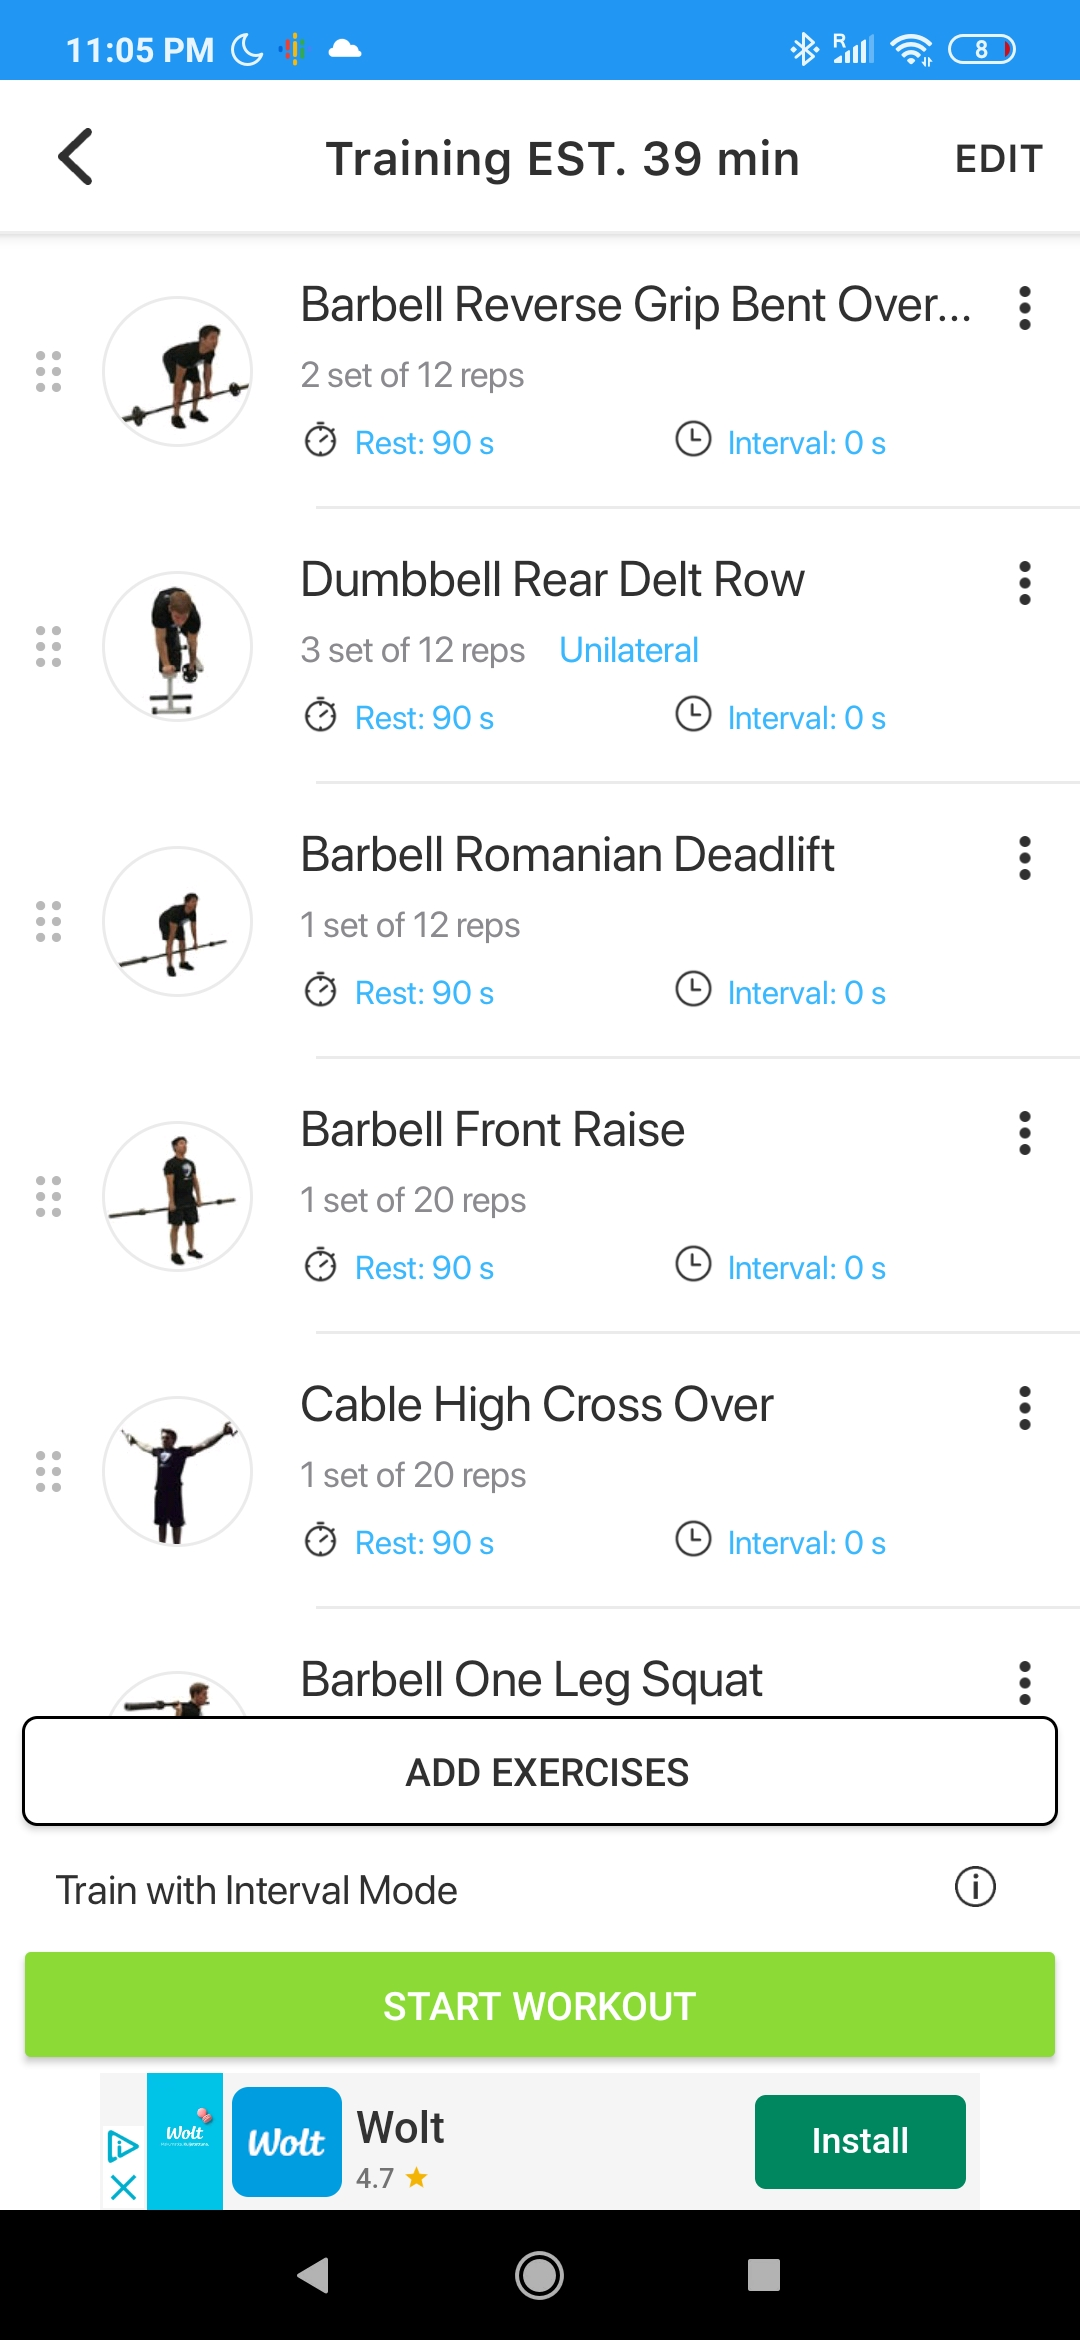
\includegraphics[width=\textwidth]{jefit_1.png}
        \caption{Jefit's interactive workout screen} 
    \end{subfigure}
    \begin{subfigure}{0.3\textwidth}
      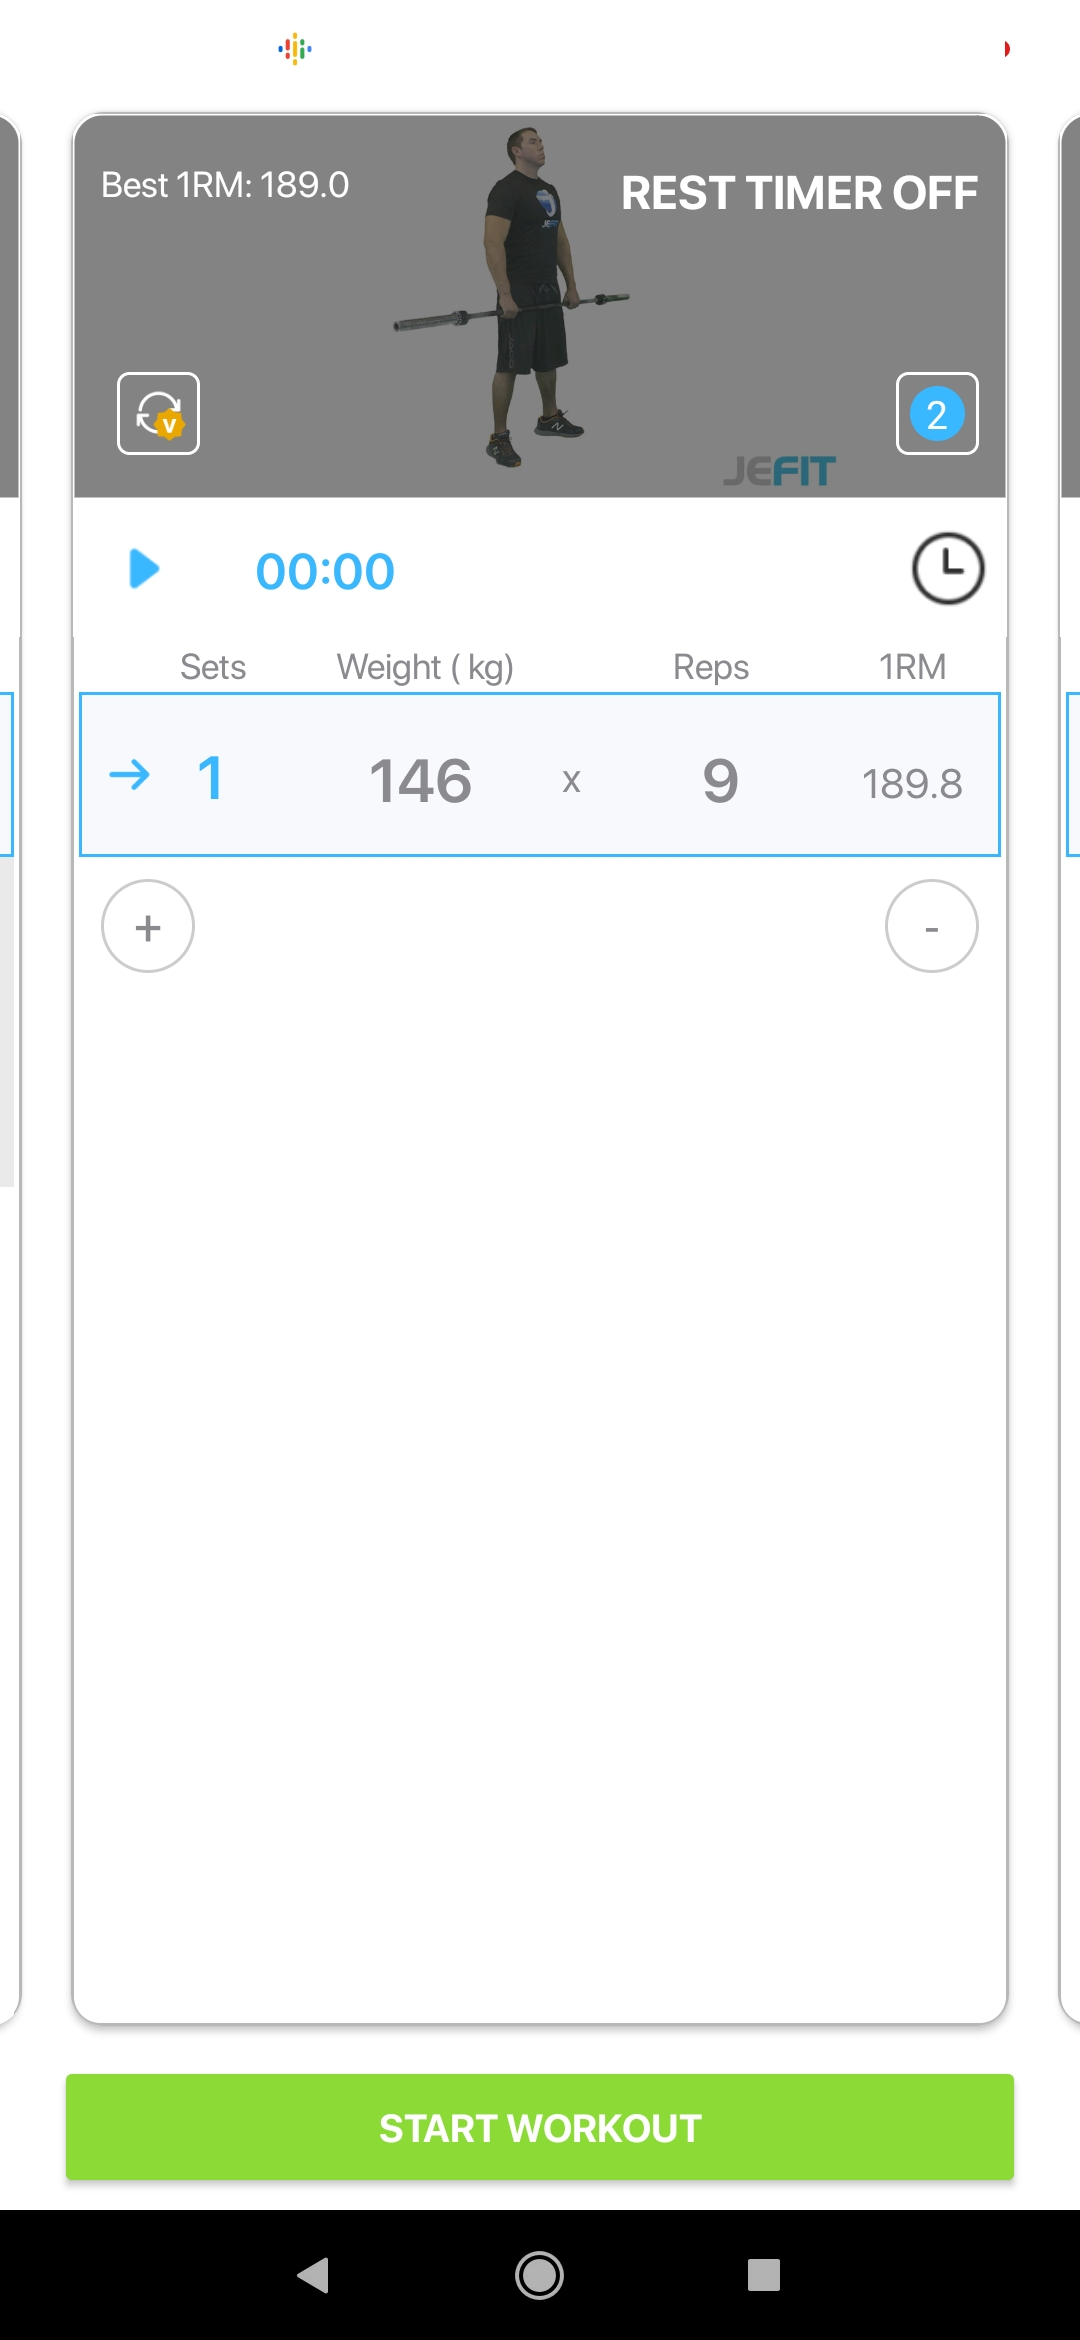
\includegraphics[width=\textwidth]{jefit_2.png}    
      \caption{The screen which is shown upon pressing on an exercise}
    \end{subfigure}
    \caption{Jefit screens}
    \label{fig:jefit}
\end{figure}

Outside of being a more restricted activity tracker, my app contains all the features of other popular trackers. 
The novel features of my app are ``Gamified Progress'', ``Collaborative Training'', ``Messaging'', and ``Friend Leaderboards''. Although other apps gave users points for working out, I didn't consider this as gamified progress as these points were just numbers with no meaning. In my app, your strength unlocks new skins and titles, and working out helps your team defeat new enemies. Although the top apps had social features, none had any form of collaborative training. Although instant messaging isn't a novel idea, none of the top fitness apps I tried had this feature. My app had a team leaderboard which was supposed to increase transparency to make use of social comparison theory. Many treated this as competitive, so I grouped my app as partially competitive.




\subsection{RPG Games}
From my analysis of RPG games, I realized that collaboration is an integral part of RPG games, and that existing products should serve as a model for implementing collaborative aspects. For instance, Clash of Clans has clans, where users need to give each other troops in order to defend one another. Clans also battle against one another in ``Clan Wars'' where users have to attack other clan's bases in order to win. Wins require members to attack consistently and to reinforce their fellow members \citep{coc}. 
Another example of a collaborative RPG is World of Warcraft. In World of Warcraft, users participate in raids together, which require very detailed coordination from all members. There are also multiple different roles which users have to take, such as healer, tank, or damage dealer \citep{wow}. There is a viral video where a World of Warcraft player named ``Leeroy Jenkins'' ruins an entire raid by going in alone as the team plans their attack, ruining their whole raid \citep{leeroy_jenkins}. Even many singleplayer RPG games are built around collaboration. For instance the game Darkest Dungeon \citep{darkest_dungeon} is built around controlling your various heroes, who can give each other status bonuses, and heal each other. For instance, the Plague Doctor hero is focused on healing others, while a Highwayman can deal lots of damage. 

From these three collaborative RPG games, I derived the following key points:
\begin{itemize}    
    \item
      Teams should fight against other players (or non-player characters)
    \item
      Users should be encouraged to help each other
    \item
      Users should have specific roles that serve some specific purpose in achieving the end goal.
    \item 
      There should be some clear progression: both on an individual level and on a collective level. Individual progression should accelerate group progression and vice versa.
    \item 
      There should be accountability: if some user(s) aren't doing their part, the team should not progress.
\end{itemize}


%==================================================================================================================================
\chapter{Analysis/Requirements}
\section{Functional Requirements}
The functional requirements state features the app could have based on the background section, and the novel features of my product.

\subsection{Must Have}

  \subsubsection{Mobile app} Almost all the existing activity from the background section were mobile apps. 

  \subsubsection{Database/server} User data needs to be stored and persisted, and should be accessible by other team members. 

  \subsubsection{Security} Users should not be able to access data which they do not have the right to access. 

  \subsubsection{Mandatory participant information/consent form }
  It is important to provide users with information about the experiment, and to get consent to use their data. I must ensure that the app cannot be used unless this form was signed.

\subsection{Should Have}
  \subsubsection{Cross platform} 
  Ideally, the app would support both Android and iOS. This will remove most technological boundaries of recruiting users. This will also make it easier for users to invite any of their friends. 

  \subsubsection{Notifications} 
  This would allow me to send workout reminders, or warn users of an enemy which is about to expire. I could also send team events, and if implemented, chat messages.

  \subsubsection{Animated characters}
  Players having animated characters and sprites makes their virtual character feel more alive. This should also make it new characters more satisfying to unlock.

  \subsubsection{Animated enemies}
  Similarly, the enemy being animated makes them feel real, and more satisfying to defeat.

\subsection{Could Have}
  \subsubsection{Websocket messaging/events}
  Events by other users would be immediately visible even without refreshing. This would allow users to chat and see what their team is as soon as this user saved the event. This is low priority, as it is only useful if two users happen to be online at the same time.

  \subsubsection{User Path Tracking}
  By tracking the paths that users take around the app, I can better understand how the app is used. This could provide some additional insight, but would mostly help to optimize my app design which is not what I am researching.


\section{Non-Functional Requirements}
Non-functional requirements are concerned with general features of the app rather than specific features.

\subsection{Must Have}

\subsubsection{Team member action transparency} 
Other members being able to see your actions allows us to leverage social comparison theory. Users want to be seen as active and helpful to the group.

\subsubsection{Personal character development}
There must be some kind personal character development. When users get stronger, it should be reflected in their virtual character.

\subsubsection{Enemy which team fights together}
In order for users to feel relatedness, they should face a common face which they fight together by exercising.

\subsection{Should Have}
  \subsubsection{Relative strength assessment}  
  When assessing the strength of a user, we should account for the weight and gender of the person. There are existing implementations, such as the Wilk's formula \citep{wilks}. This allows more diverse participants to compete.

  \subsubsection{Warnings for users progressing in weight too quickly} 
  This is important to prevent injuries, and to ensure that my research does not endanger participants.

\subsection{Could Have}
  \subsubsection{Out-group competition}
  Some kind of leaderboard would encourage competition between teams. Although I think this would be motivating, I am not investigating out-group competition.

  \subsubsection{Live workout tracking}
  Users could enter their performed exercises as they complete them at the gym.




%==================================================================================================================================
\chapter{Design}
A key feature of collaborative activity trackers is that exercise must have some collective benefit beyond just the individual benefit. I implemented this through users fighting an enemy together, such as in World of Warcraft raids. User damage is calculated through their strength as well as their effort. 

\section{Calculating a User's Contribution to Their Team}
I wanted this app to calculate your team's contribution based on your effort and your strength. Rewarding effort should hopefully motivate users to work out regularly and push themselves, even when progress plateaus. Progress is rarely linear: it often has bumps, but through perseverance, you move more forwards than backwards. This also motivates users with lots of experience as they can often feel demotivated by the waning progress, and the amount of time and effort it can take to accomplish something a beginner can achieve in a fraction of the time. I also reward strength progression, as I want the app to provide users with long term motivation, and to motivate users to train for results and not just for the sake of training. Rewarding progression also discourages overtraining. If I only reward effort, the optimal strategy would be to exercise as much as possible, even if you felt pain or your progression stopped and regressed. By rewarding strength improvements, I reward the user for training moderately and resting adequately, as these are integral for long term progress. I gamify strength as attack damage, and effort as the number of attacks you deliver towards your team's enemy. The product of the two is the total damage that you deal towards your team's enemy. This total damage is dealt towards the monster that your enemy is currently fighting, and represents a member's contribution to the group.

Initially I had to quantify strength, or attack damage. I wanted strength to be calculated relative to the person performing it. For example, it is harder for an average 50 kg person to lift the same weight as an average 80 kg person. By taking this into account, I made the app more inclusive, and allowed everyone to contribute based on how strong they are relative to others like them, and not everyone else. For every exercise, users were asked to input their repetitions and weight. Using this information and the provided gender and bodyweight of the user, I was able to estimate the relative strength of this user for that exercise. There are sites which perform this calculation, which I will go into more detail in section \ref{strength_calculations}. I was still left with the challenge of converting per-exercise percentiles into a single strength value. Initially I used a simple naive implementation which took the mean percentile of all exercises, and used that as the final strength value. This is problematic, as this would encourage users to only track their best exercise, and nothing else. I don't want my app to encourage users to just focus on one exercise, as this can lead to injuries and imbalances. With this in mind, I decided that users should be rewarded for adding more exercises up to a certain number by setting strength to be the product of the average strength and the total number of tracked exercises. This seemed good, but this simplified to be just the sum of percentiles.

\begin{algorithm}[H]
  $\frac{\sum_{i=0}^{n} x_i}{n} * n = {\sum_{i=0}^{n} x_i}$
\end{algorithm}

I only realized this on the first day of the evaluation. Luckily, this was a simple database function, so it was easy to replace this calculation. 
My final solution was to multiply the average strength percentage with the number of exercises log scaled, which only rewarded adding more exercises up to a certain point. I think it's important to discourage laborious strategies such as keeping track of 50 exercises just because it would increase your total damage. 

\begin{algorithm}
  $attack\_damage = \frac{\sum_{i=1}^{n} x_i}{n} * ln(n) $

  where the user has tracked $n$ exercises, and $x$ contains the strength percentiles for exercises 
\end{algorithm}

Next, I had to decide how I would grant attacks based on workout effort. I could compare the user's per exercise performance relative to the last time. This would have a lot of confounding factors: personal differences and skill level let some add more weight with less effort. There would also be the problem of missing data (what is the effort on your first workout, or when you use new exercises?). This would also require users to input the number of repetitions and lifted weight for all their sets for all their exercises. Finally, this wouldn't reward users for putting in effort even on a bad day or during a plateau. I consulted sport science literature, and found a popular metric for estimating effort is called ``RPE'' (Rate of Perceived Exertion). RPE is a scale from 1-10, where 1 is almost no effort, 5 is moderate effort, and 10 is maximal effort. RPE has the downside of not being objective, as we are relying on a person's subjective perception of their effort. Research by \citet{RPE_estimations} found that ``The odds of underestimating RPE for an exerciser were 3.67 times greater than a non-exerciser''. This could be offset by reducing the RPE that beginner's estimate, but this was out of scope for this project. I am not particularly worried about intentional dishonesty regarding RPE, as users can lie about the number of sets they complete, how much they can lift, how often they train, etc. I decided to use RIR (repetitions in reserve), which is an inverse of RPE as it seemed easier to understand than RPE. The article by \citet{rir} made a good case for measuring total training stress through average RIR and total sets. I couldn't find any specific equations that combined the two, so I created this equation, which increases as average RIR decreases and total sets increase.

\begin{algorithm}
  $granted\_attacks = min(0, 10 - average\_rir) * total\_sets)$
\end{algorithm}

With both attack\_damage, we can write the damage dealt by a workout as 

\begin{algorithm}
  $workout\_damage = attack\_damage * granted\_attacks$ 
\end{algorithm}


\section{Communicating App Functionality to the User}
One of the big challenges was implementing strength exercise tracking which was understandable, yet quick to use. My solution minimized input: you could voluntarily update exercise personal bests whenever you got a new record, and track workouts by entering the total number of exercise sets along with how difficult they were on average. The downside of this was that it resulted in two screens. 

When you open the app, you initially see two buttons on the top labeled as ``Strengthen Character'' and ``Deal Damage''. ``Strengthen Character'' lets you update your exercise personal records, which increase your character's strength. ``Deal Damage'' on the other hand lets you track a workout, which deals damage towards your team's enemy. I decided to label these based on the effect that these actions have in game, as opposed to ``Update Exercise'' and ``Track Workout'' which I initially used. This is because I believed that the required real life data input could be easily inferred from these screens, so it would be a good opportunity to help the user understand the real life connection to the game. If a user clicks on ``Strengthen Character'', and they see a screen that allows them to input their exercise performances, I would hope that they would understand that in-game strength is calculated through your real life strength. 

\begin{figure}[H]
    \begin{subfigure}{0.45\textwidth}
        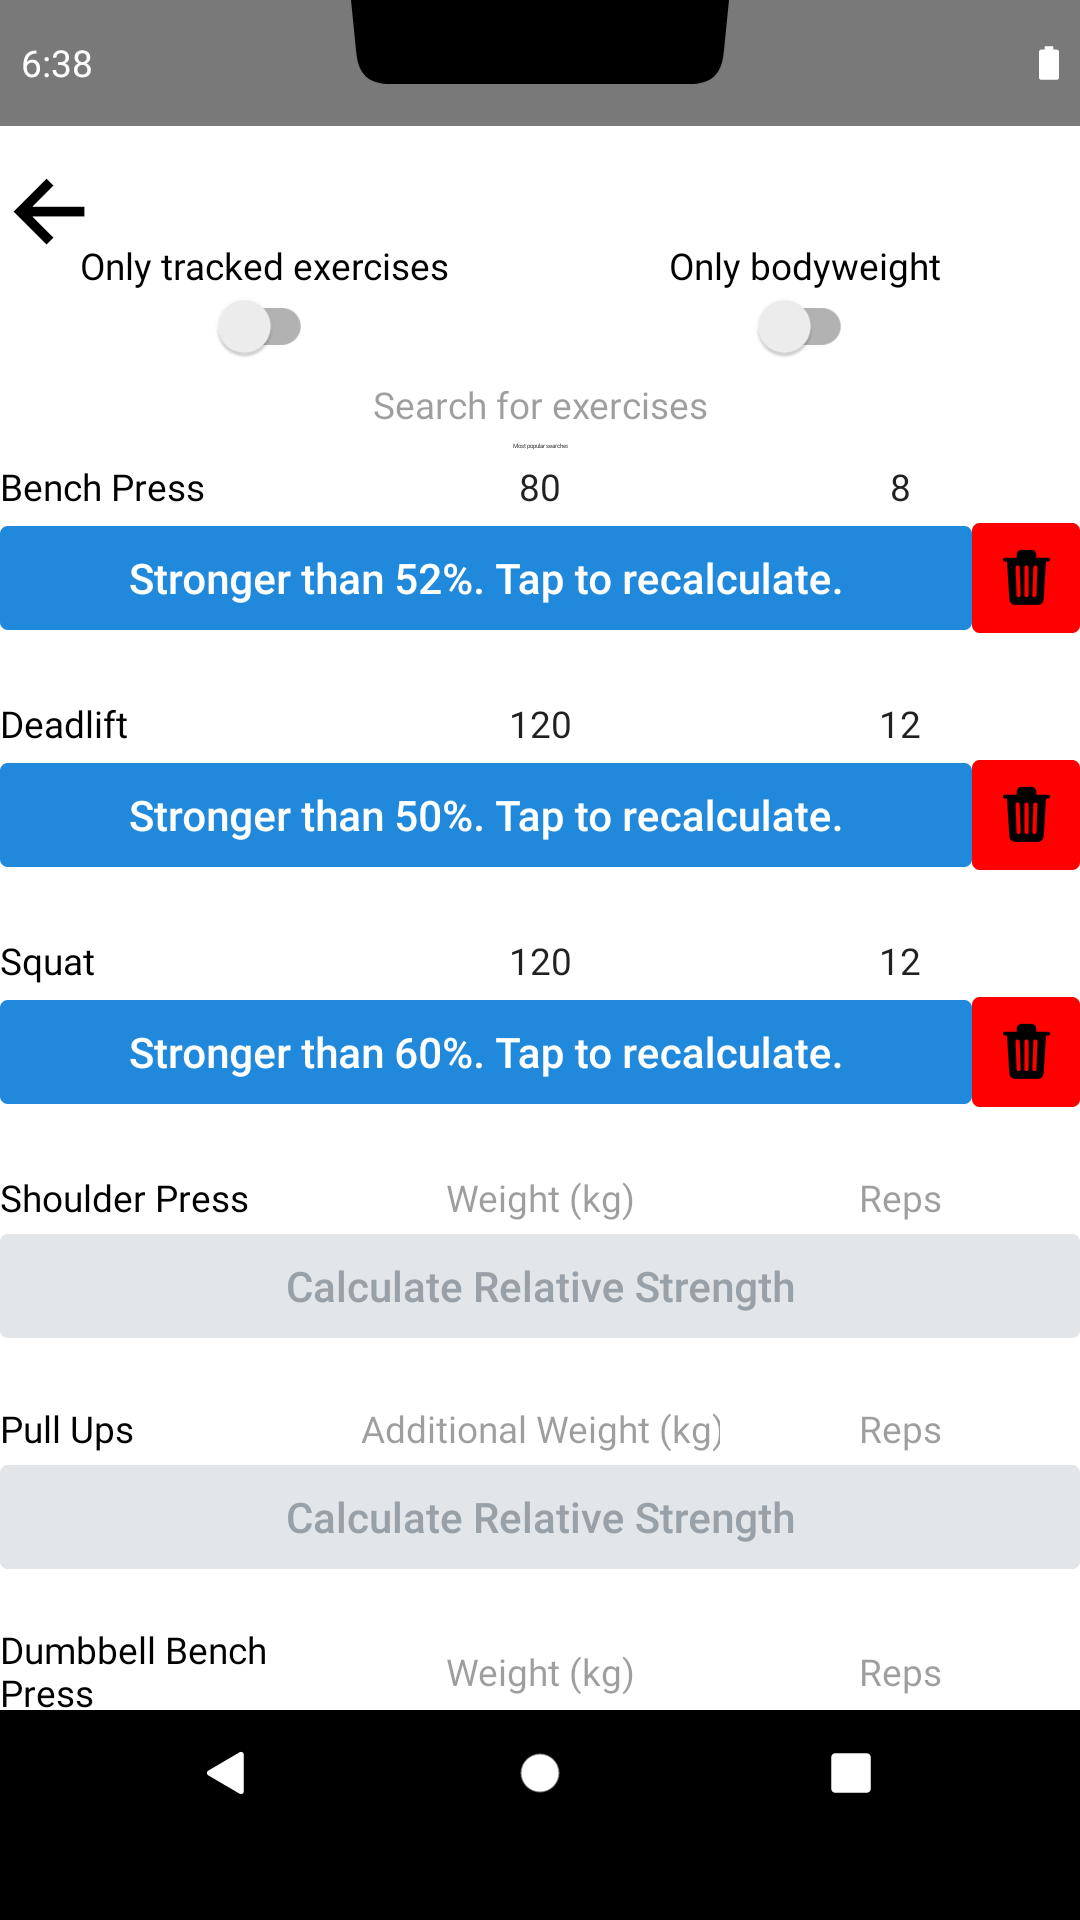
\includegraphics[width=\textwidth]{exercise_modal.png}
        \caption{``Strengthen Character'' screen} 
    \end{subfigure}
    \begin{subfigure}{0.45\textwidth}
      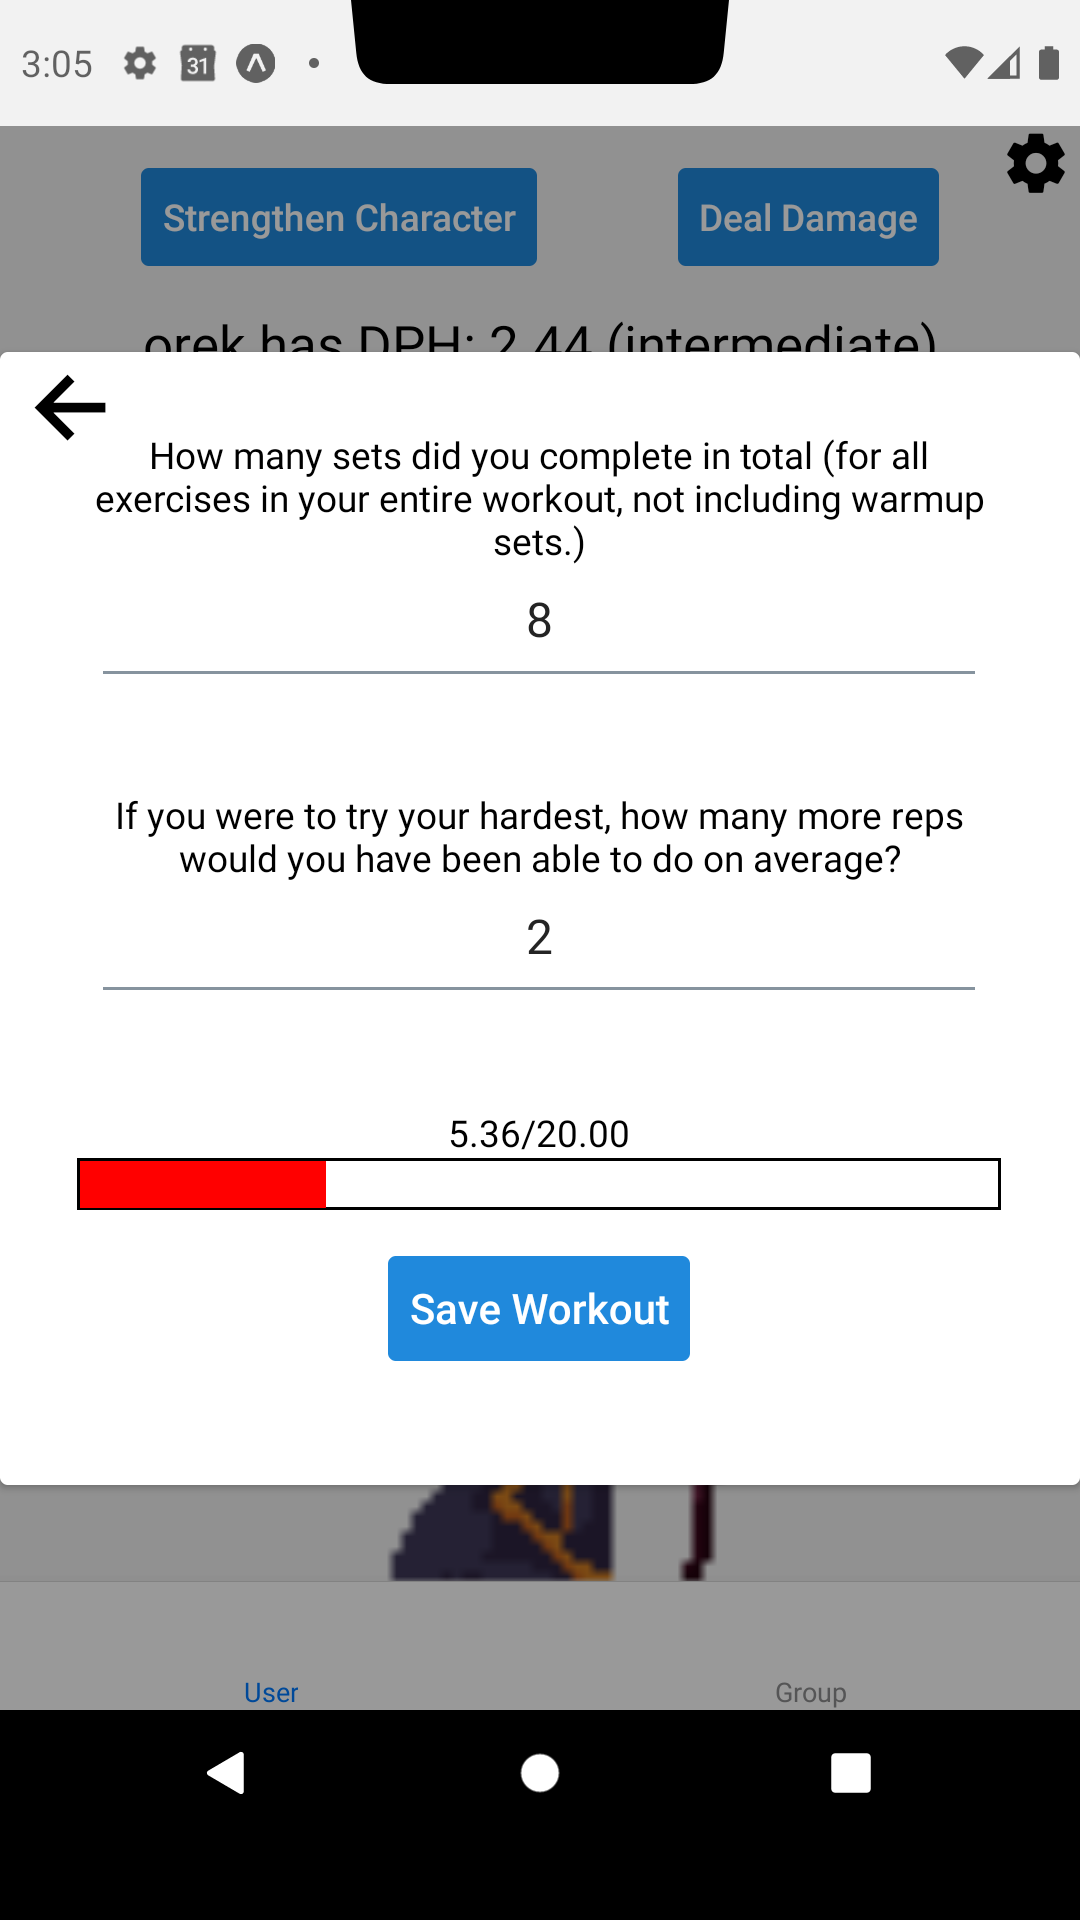
\includegraphics[width=\textwidth]{workout_modal.png}    
      \caption{``Deal Damage'' Screen}
    \end{subfigure}
\end{figure}

The right-hand ``Deal Damage'' screen is far more verbose than the left-hand ``Strengthen Character''. When I was running my pilot study, I found that participants instantly understood that they were being asked to input how many repetitions of a weight they could do on a given exercise. Users were more confused with the idea of total sets, as they weren't sure what constituted as a set. Users also struggled to understand what ``reps in reserve'' were. I added the explanations above each requested value to help explain these.

\newpage

The extra manual work of tracking strength training was also an opportunity to give the user instantaneous satisfying feedback. When a user closes the ``Strengthen Character'' screen after adding exercises, their attack damage changes. If their attack damage reaches a new threshold, the character look also changes. I wanted everyone to experience this when tracking their first exercise(s). As long as you track a single exercise and make your attack non-zero, you get a new character.

\begin{figure}[H]
    \begin{subfigure}{0.45\textwidth}
      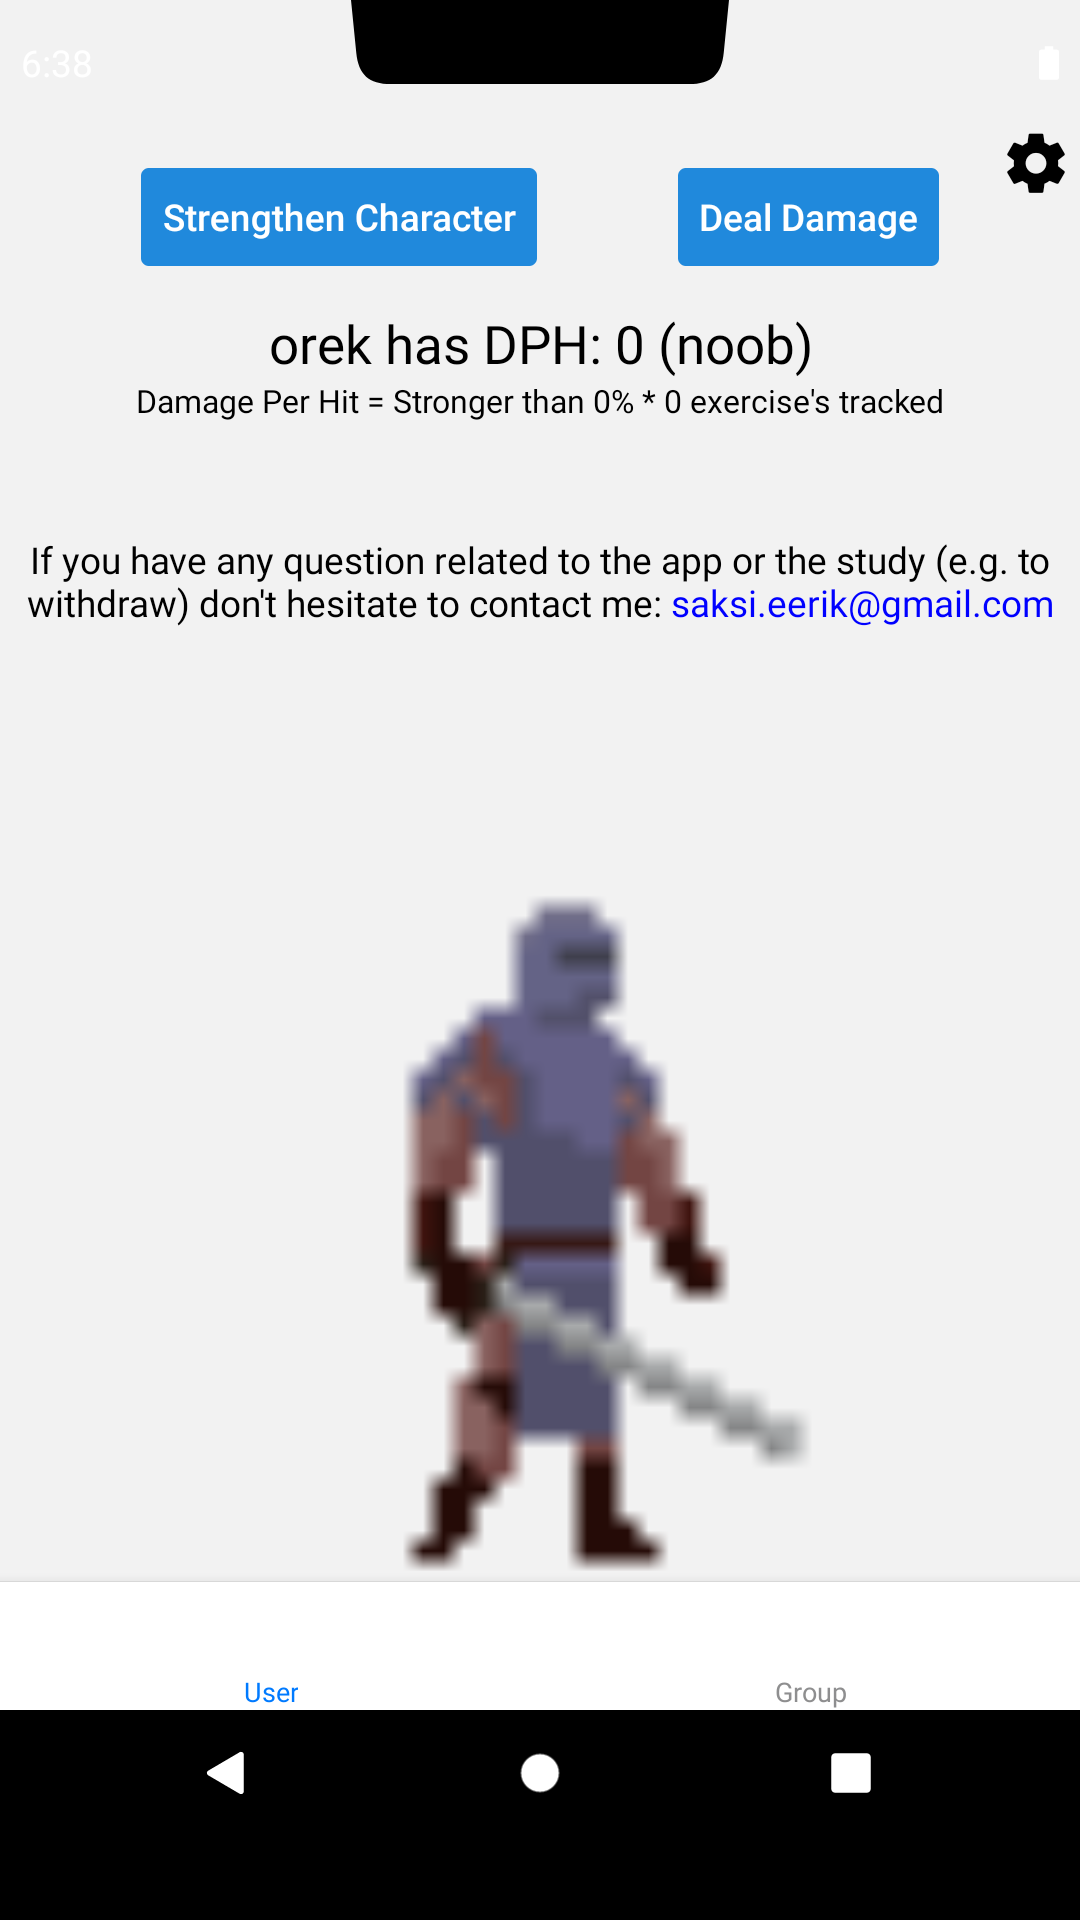
\includegraphics[width=\textwidth]{noob_user_page.png}    
      \caption{What the user sees initially}
    \end{subfigure}
    \begin{subfigure}{0.45\textwidth }
        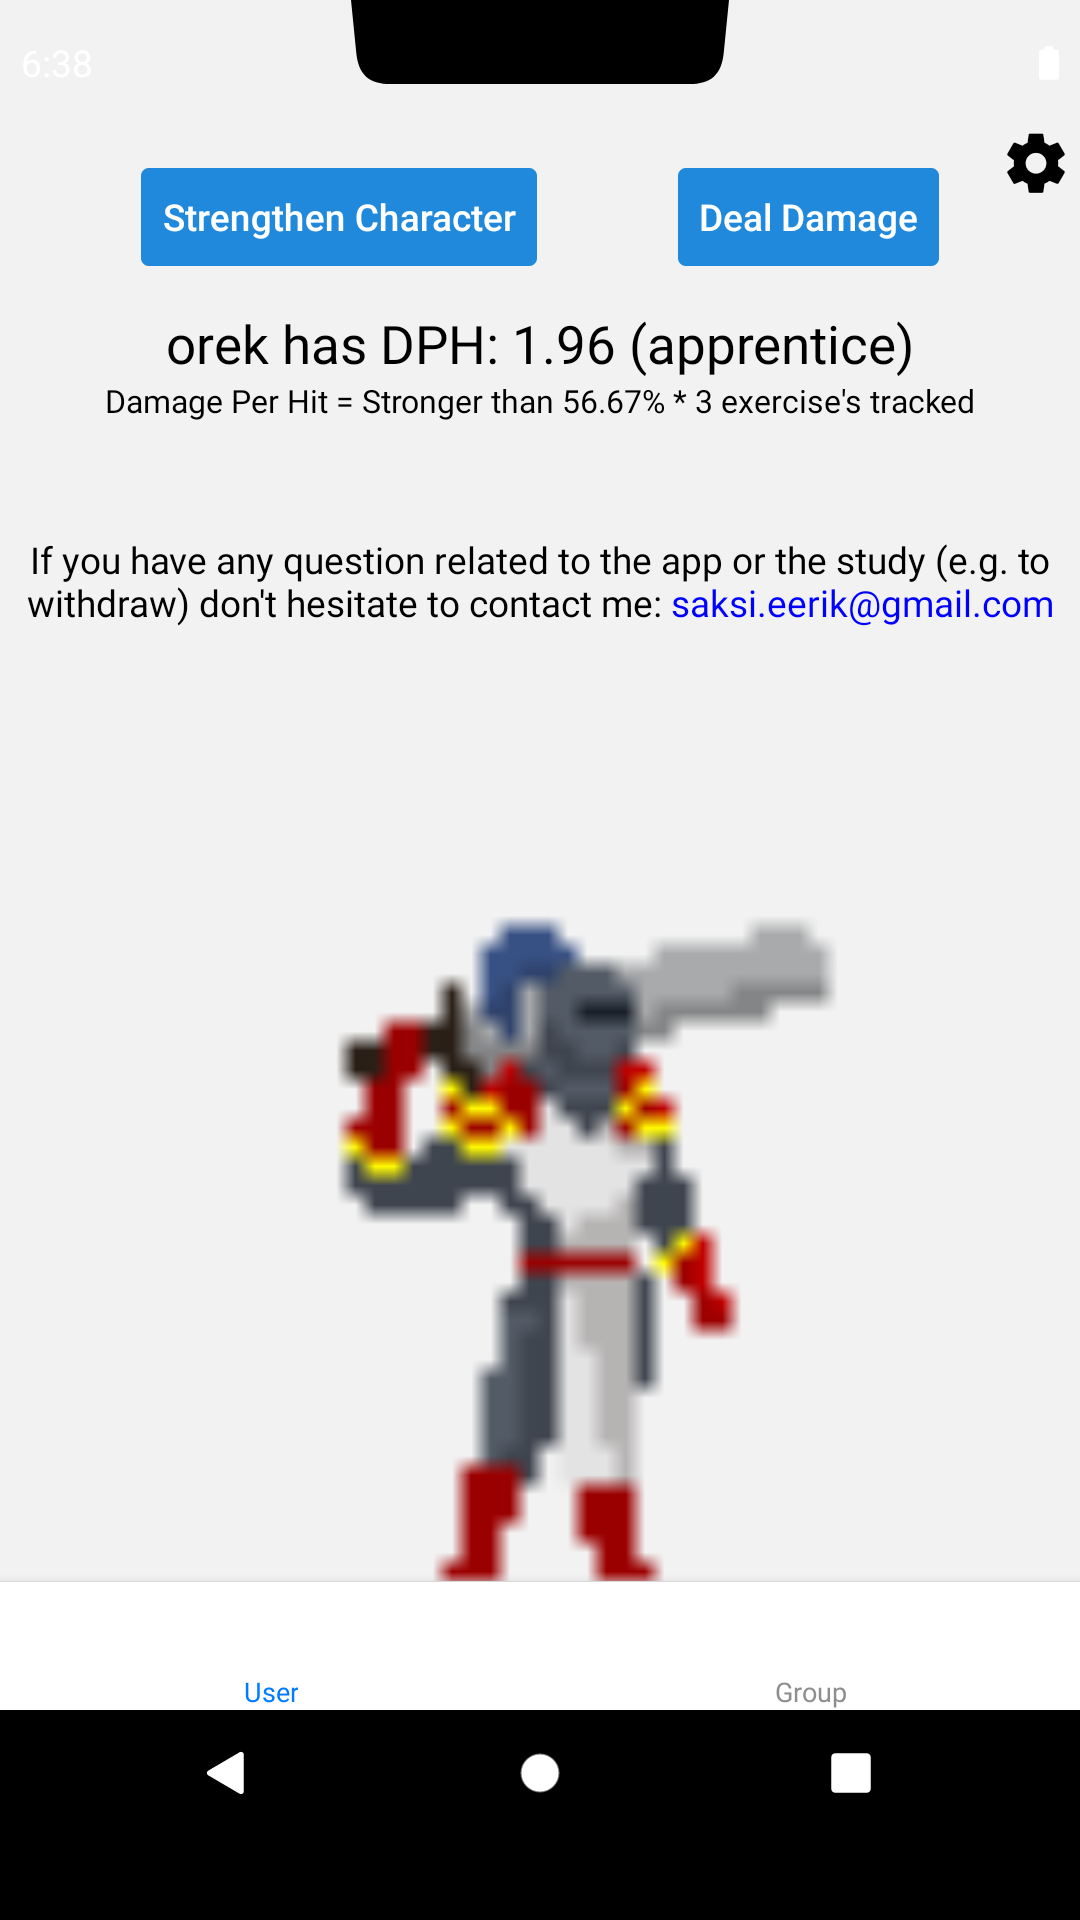
\includegraphics[width=\textwidth]{apprentice.png}
        \caption{What the user sees after tracking 1 or more exercise} 
    \end{subfigure}
\end{figure}

\newpage
I also tried to make tracking workouts feel satisfying. After saving the workout, the user initiates a fight with your team's enemy. The user gets to see the animations of your character attack, and the enemy take damage, one hit at a time. This is skippable, as it might become boring for long-time users. Killing the enemy will also trigger a dying animation from the enemy.

\begin{figure}[H]
    \centering
    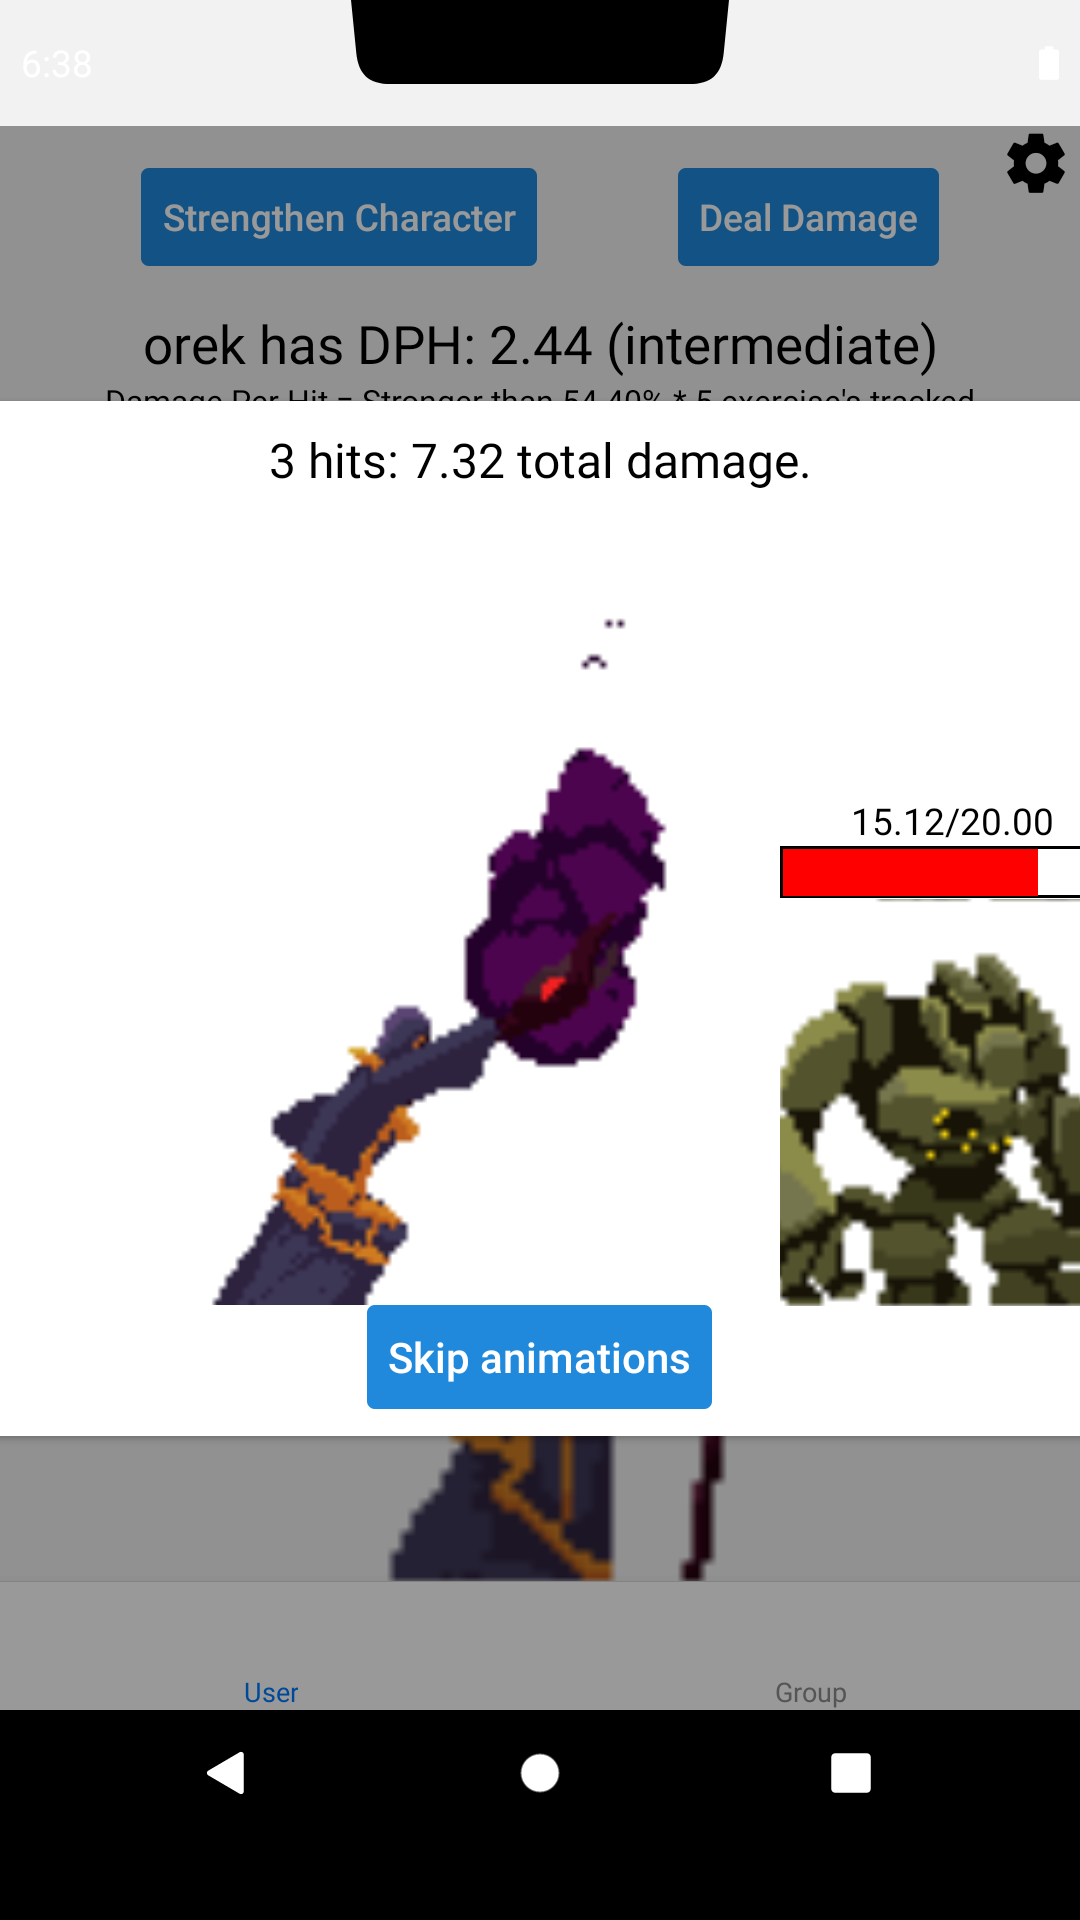
\includegraphics[width=0.7\linewidth]{attack.png}    
    \caption{ An active battle. There were some visual bugs that I didn't have time to fix.  }
\end{figure}

\newpage

I also created a tutorial that explains this idea further. This tutorial is shown when you initially launch the app. In order to demonstrate the connection with real world strength and in-game strength, I change real world strength inputs and show the in-game character get stronger.

\begin{figure}[H]
    \begin{subfigure}{0.45\textwidth}
      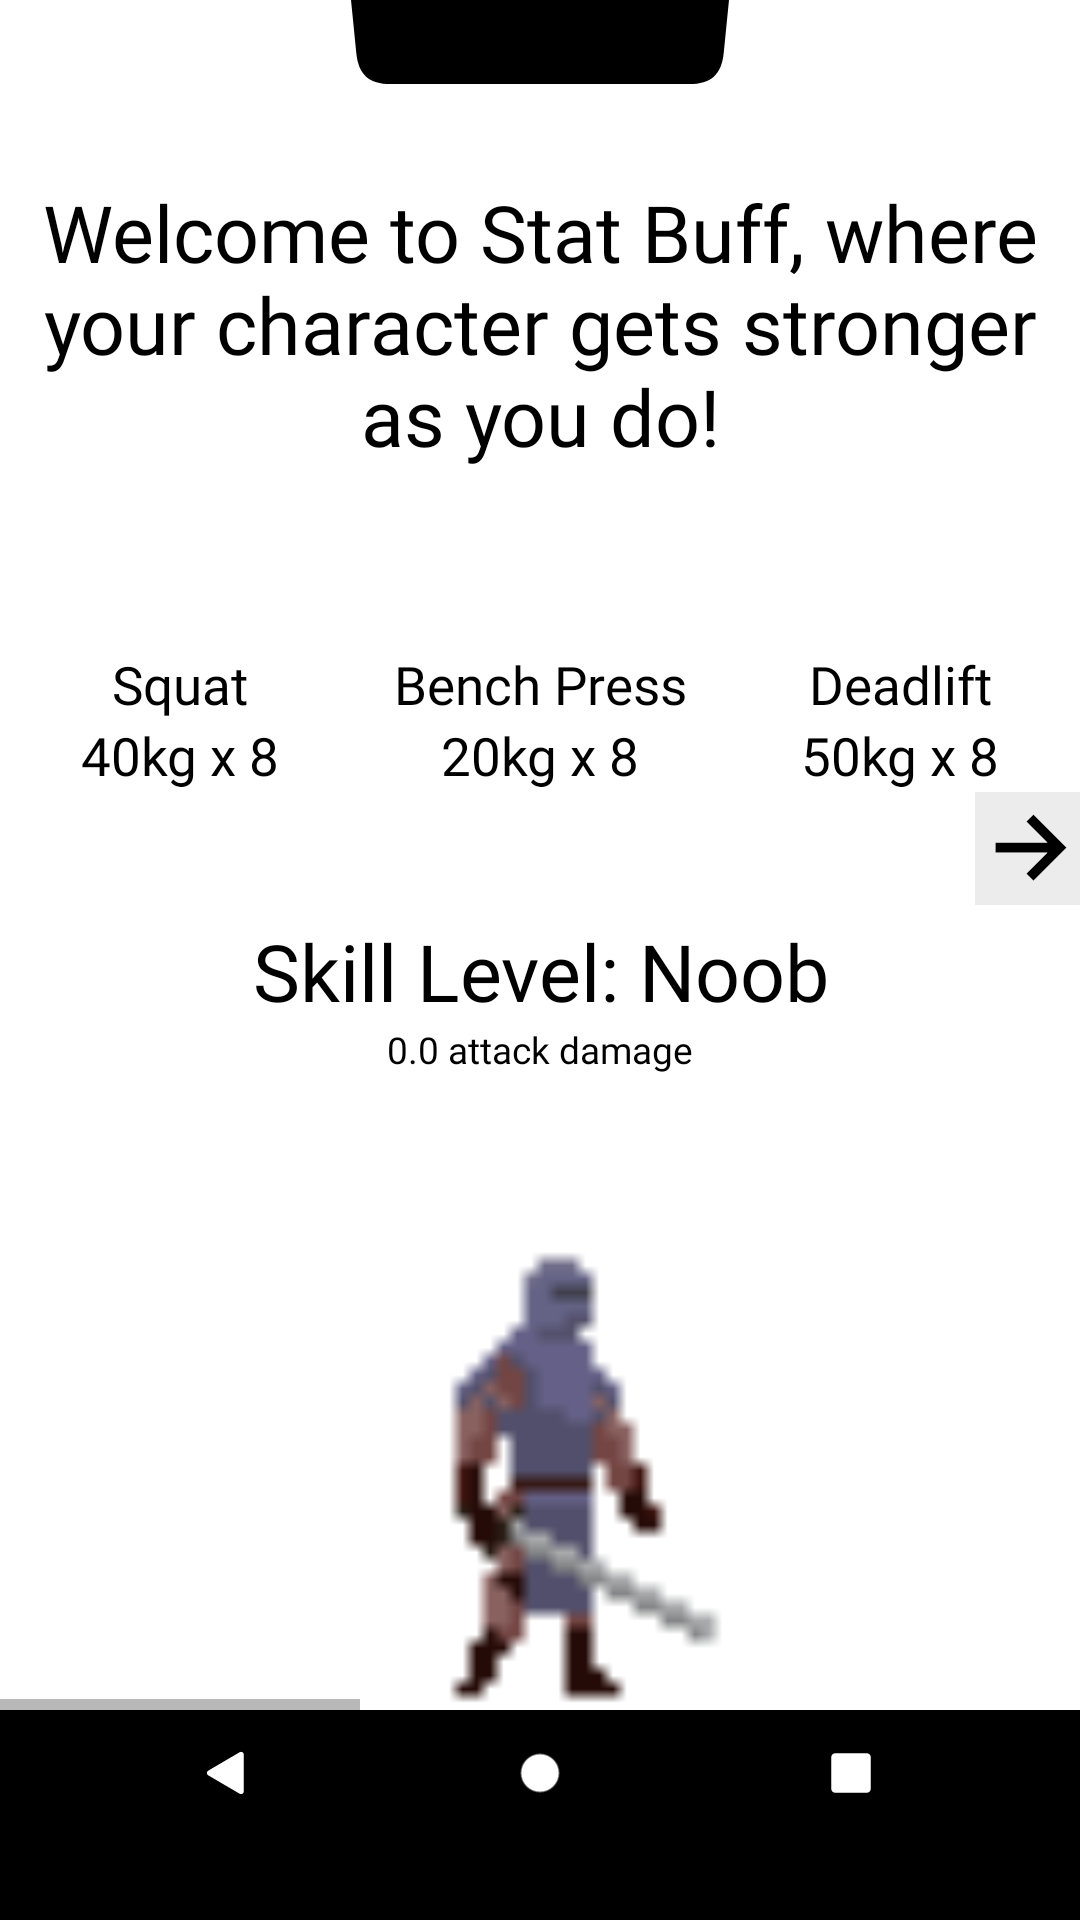
\includegraphics[width=\textwidth]{noob.png}    
      \caption{The ``noob'' character is shown due to the low strength values}
    \end{subfigure}
    \begin{subfigure}{0.45\textwidth}
        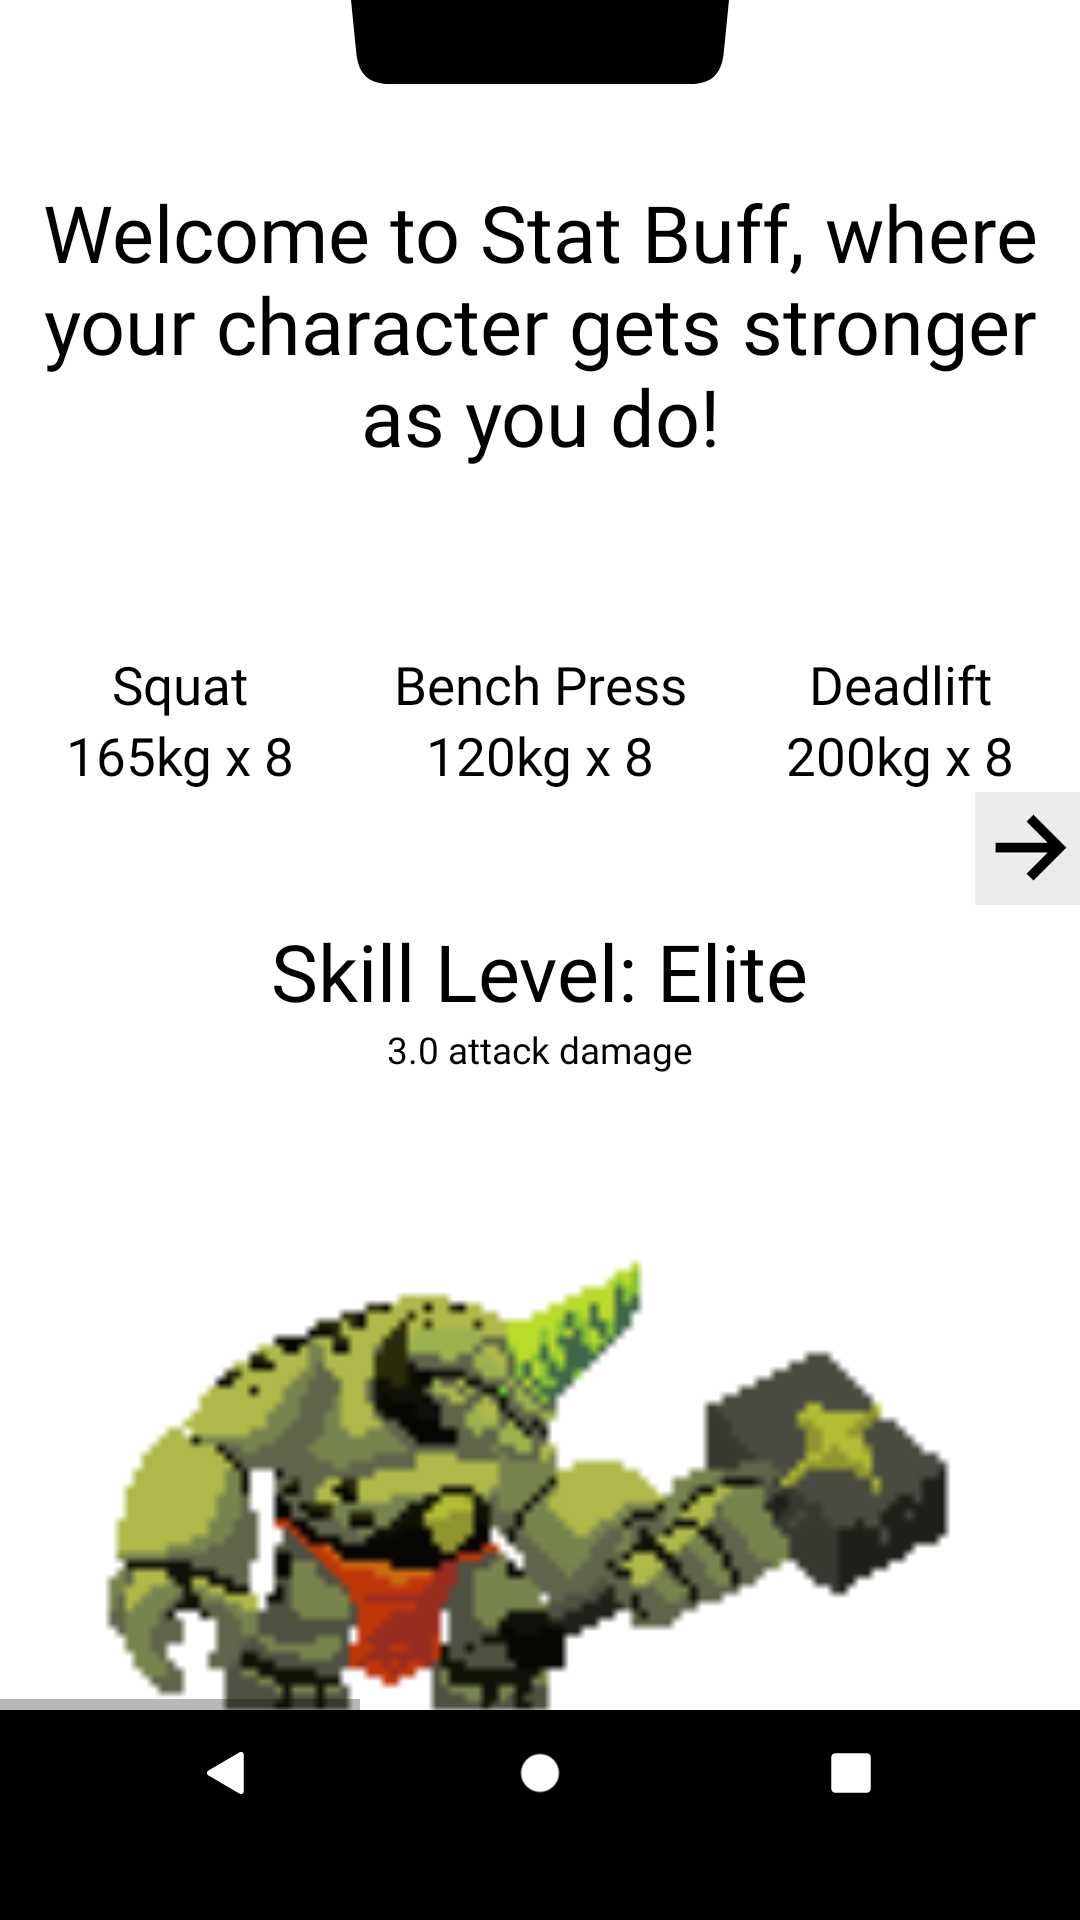
\includegraphics[width=\textwidth]{elite.png}
        \caption{The ``elite'' character, unlocked through high real world strength} 
    \end{subfigure}
\end{figure}

\newpage
In order to demonstrate how workouts deal damage towards an enemy that you fight with your friends, I show two different characters taking turns fighting a monster, where the second player finishes the monster off.

\begin{figure}[H]
    \begin{subfigure}{0.45\textwidth}
      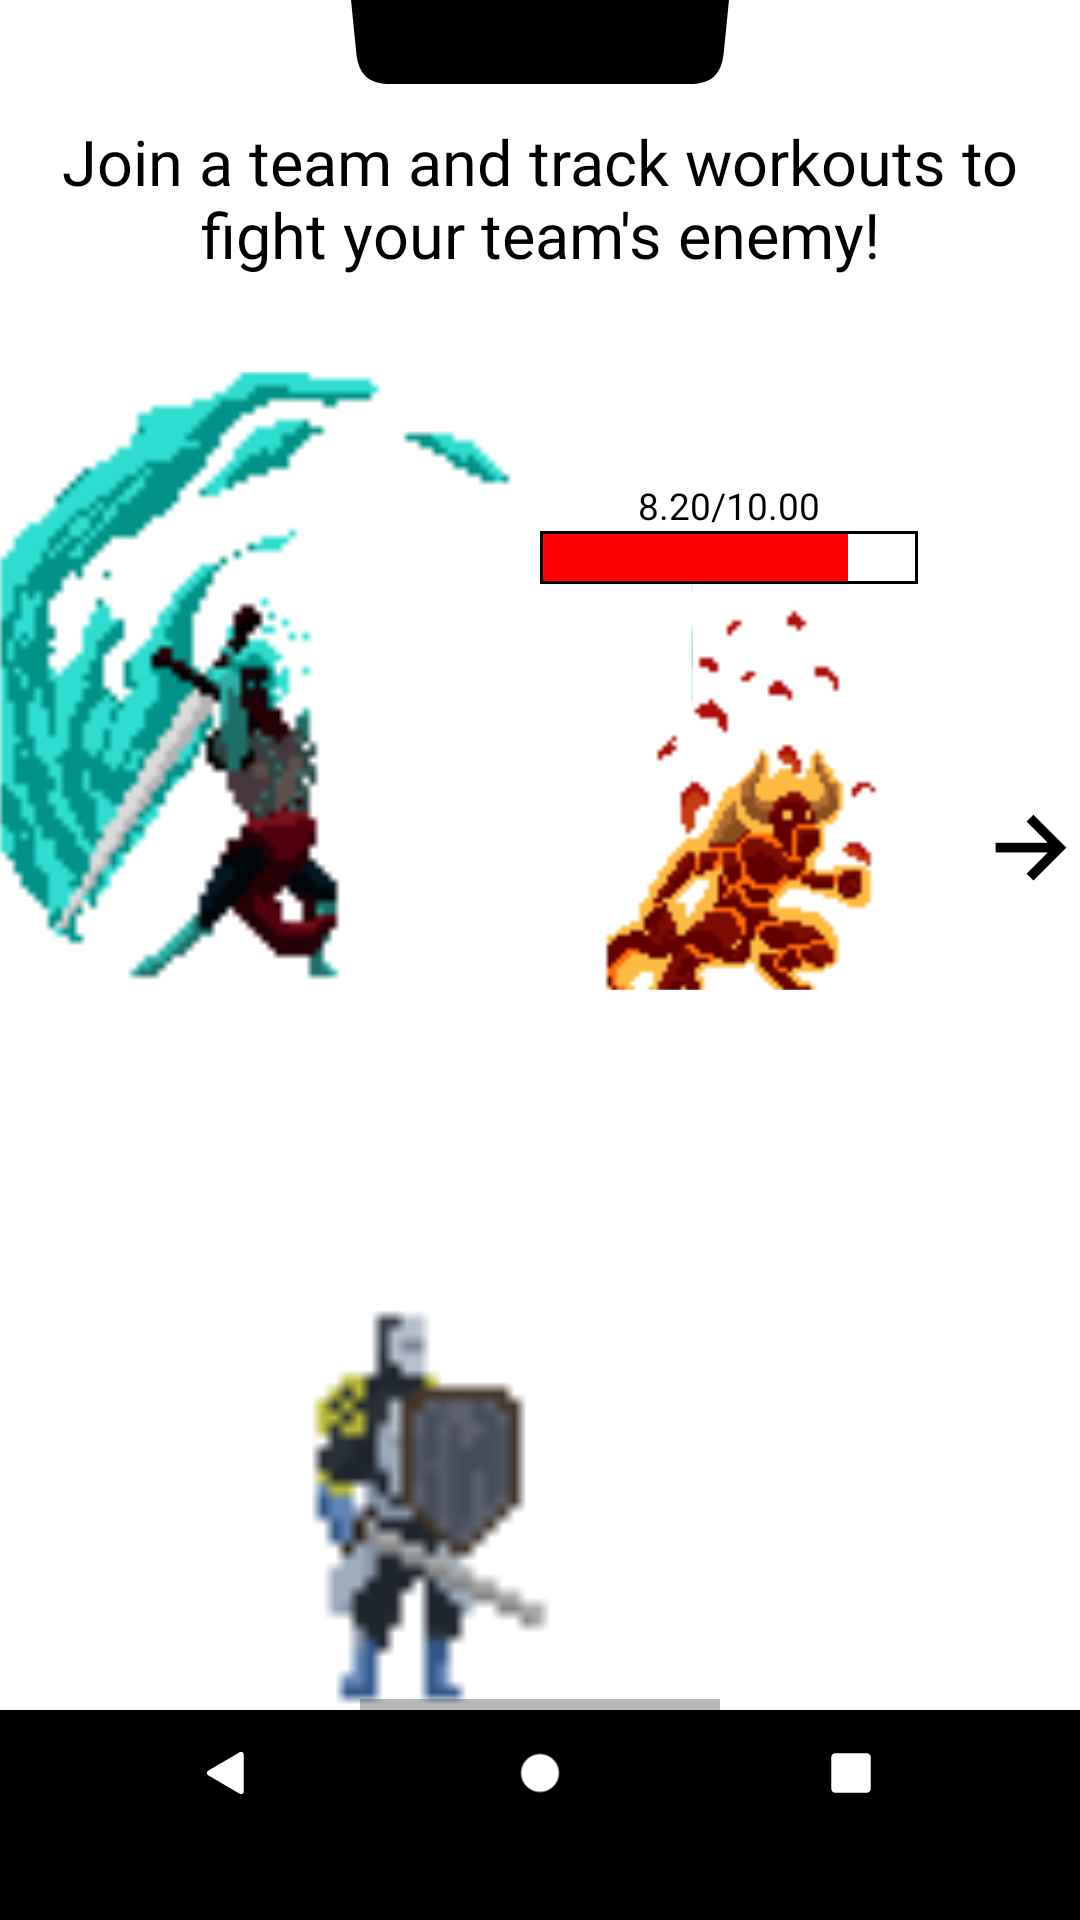
\includegraphics[width=\textwidth]{upper_attack.png}    
      \caption{The first player deals initial damage to the enemy}
    \end{subfigure}
    \begin{subfigure}{0.45\textwidth}
        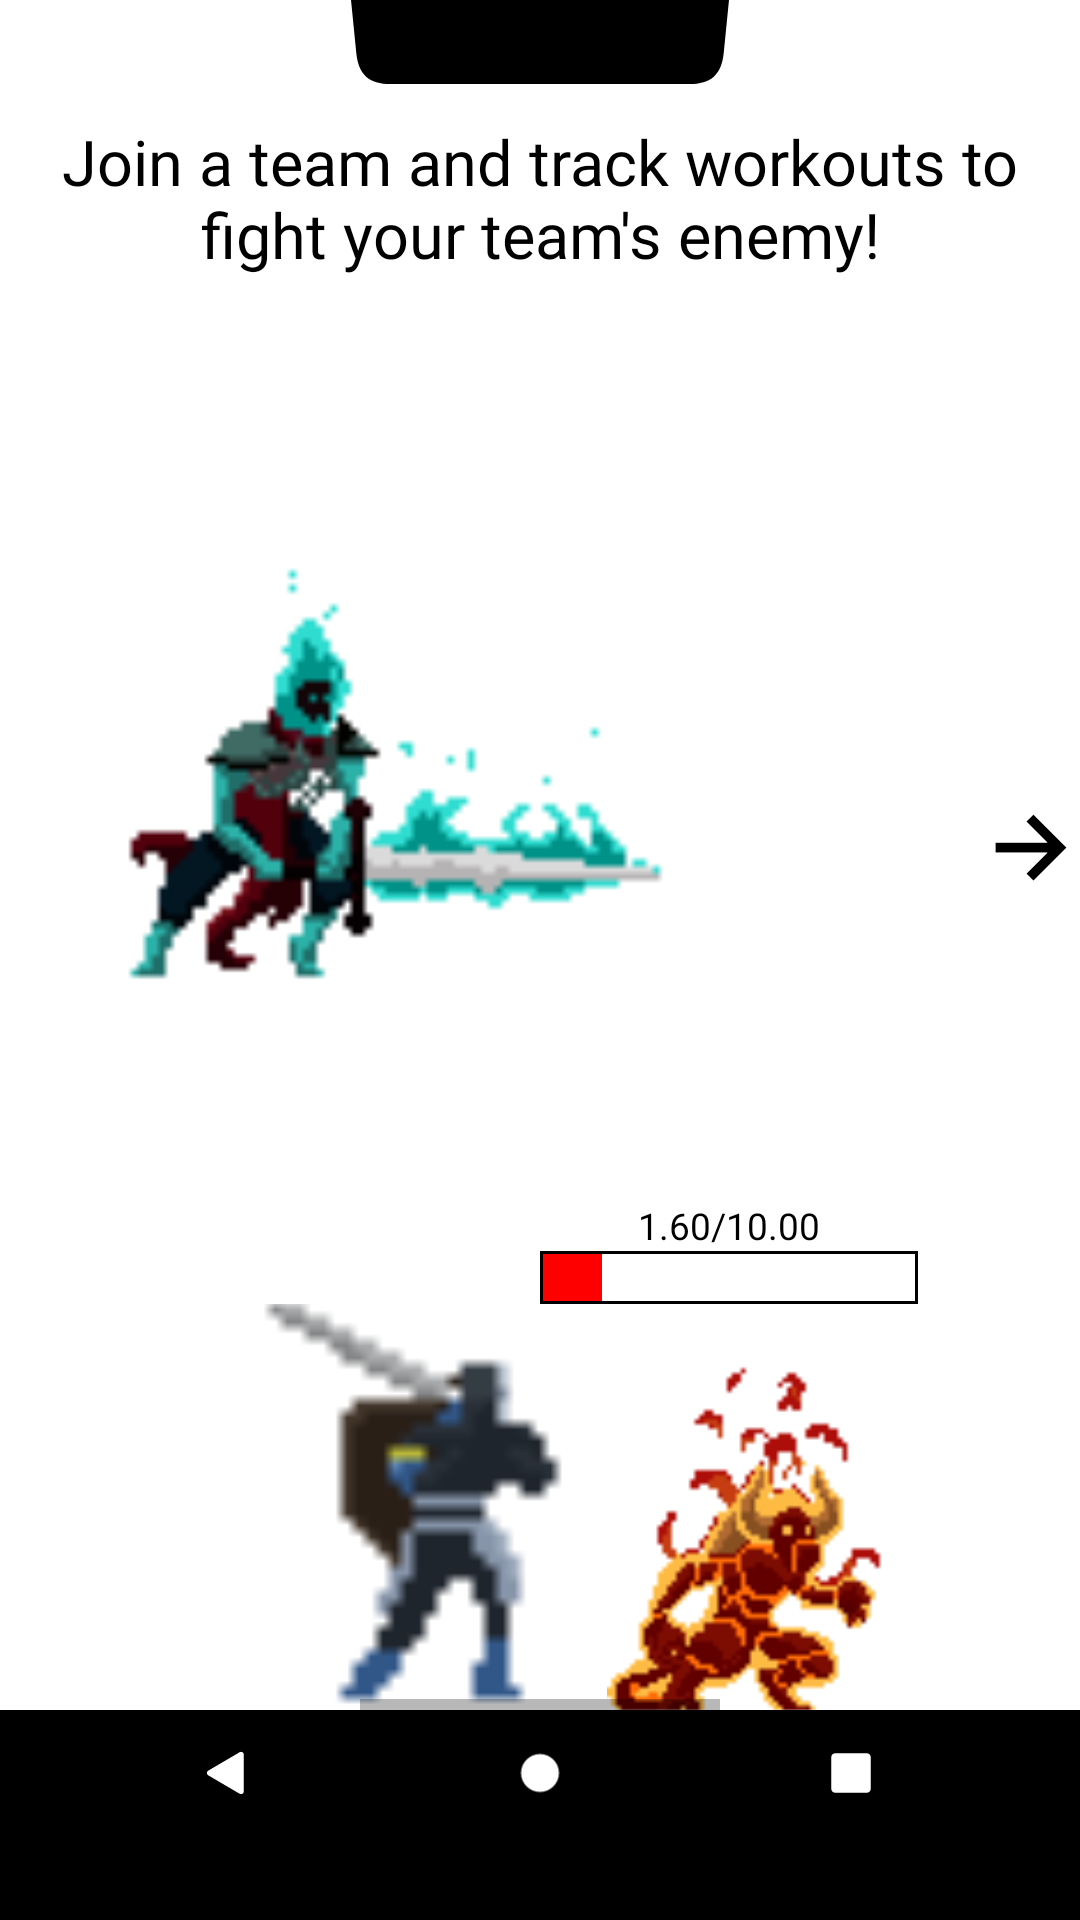
\includegraphics[width=\textwidth]{lower_attack.png}
        \caption{The second player then kills the wounded monster} 
    \end{subfigure}
\end{figure}

\section{Enhancing Collaboration With Research} \label{enhancing}
In order to make collaboration as useful as possible, I had to apply some of the techniques I covered in the background. One of the three mini theories of self determination theory is social relatedness. I tried to leverage social relatedness through creating a single enemy that users fought together. Winning or losing against this monster was a reflection on the exercise habits of the entire team. Users could celebrate a victory against their common enemy, or plan how they would defeat the monster the next time.

Argues that people change behaviour based on how they are viewed by others. I leveraged this by adding high transparency towards the actions of other users. I added a timeline which contained all team member events, such as workouts or new personal bests. There was also a tab which showed the total contribution of all users over time, as well as for specific battles. Users are motivated to exercise, as they know everyone will see them contribute to the team. There is also negative enforcement, as users don't want to be seen as slackers by other team by being in the bottom of the team's leaderboard. You can see a screenshot of the chat in \ref{fig:chat}.

Social support theory argues that positive social encounters are positive. I added a simple real-time chat which allows users to talk amongst themselves. I tried to add discussion topics which would increase the likelihood of positive interaction. Through the time limit to defeat enemies, users were encouraged to discuss their training plans amongst themselves to better coordinate battles. I also tried to add some humorous monsters to the game to elicit reactions and discussion, such as Figure \ref{fig:frogman}. 

\begin{figure}[H]
    \centering
    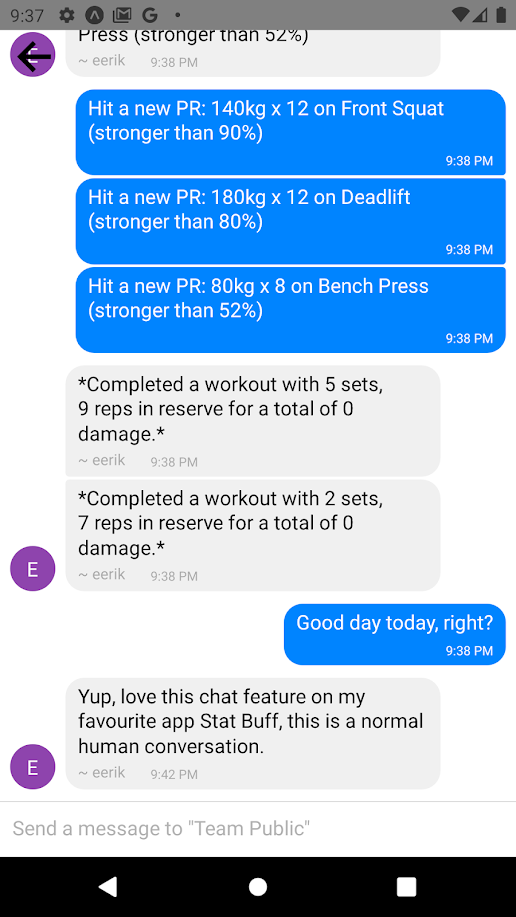
\includegraphics[width=0.4\linewidth]{chat.png}    
    \caption{The chat and timeline of a fictional group}
    \label{fig:chat}
\end{figure}


\begin{figure}[H]
    \centering
    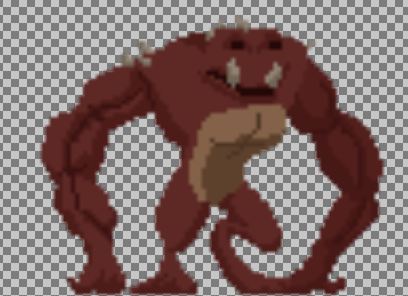
\includegraphics[width=1.0\linewidth]{froggie.png}    
    \caption{
      ``Frogman, the King of Deadlift Leverages. The deadlift is performed by picking up the weight from the ground, so this frog has great leverages for the exercise.''
    }
    \label{fig:frogman} 
\end{figure}

\chapter{Implementation}

\section{Technologies Used}
%rds, heroku, graphql, apollo, react 
I first had to choose a technology that I would use to build the client. I decided that an app would be more convenient than a website, as users could enter values during/right after exercising. After deciding to make an app, I had to decide which platform's to develop for. Ideally, I would have an app for both platforms, which would allow anyone to participate. Participants could also invite any of their friends. I didn't have time to learn how to make an iOS app and an Android app, so I decided to make a single React Native app, which can be compiled into two native apps. I also had some experience with React, which made learning React Native easy. All of my React Native code was written in Typescript. Typescript is only a development dependency, and isn't bundled into the app itself. It is compiled into Javascript during the build phase. Typescript comes with type enforcement and built in null/undefined checks which makes catching bugs much easier. 

As the app was collaborative, I needed to set up a server and a database. I wanted to make this as easy as possible, so I used a technology called Postgraphile, which turns a Postgres database into an API automatically. Postgraphile only translates user requests into SQL queries and SQL query results into server responses. Security rules and more complex logic was implemented in Postgres. I hosted the server on Heroku, and used an AWS relational database server. 

I used a library called Apollo in order to interact with the server from the client. This made it easy to set up caching, interface updates on data update, and websocket subscriptions. 

I also hosted a participant information/ethics consent form written in React on my Heroku server. Users who tried to sign up but hadn't signed the form would be taken to the site. Once the form was signed, the website would reopen the app, which refetched the status of the consent sheet. If this was ok, users would successfully sign up.

\section{Server/Database implementation}

The server is built with a technology called GraphQL. GraphQL is a query language similar to REST, except GraphQL requests require you to pass a JSON-like object containing only keys for which you want the values for. This is what a simple GraphQL request might look like: 

\begin{lstlisting}[language=python, caption={An example GraphQL query fetching a user's group}, label=lst:callahan]
  query{
    user(username: "orek"){
      groupname
    }
  }
\end{lstlisting}

\begin{lstlisting}[language=python, caption={Response to above query}]
  {
    "data": {
      "user": {
        "groupname": "Team Public",
      }
    }
  }
\end{lstlisting}
This query format has many benefits: a well configured client would never overfetch or underfetch. In a standard REST setup, the /user endpoint might return user metadata and /messages might return a users messages. This would mean that the client would have to send two requests, which would be slower for both the client and the server. One solution might be setting up a single endpoint, /user\_messages, which returns both user metadata and user messages. This would have the downside of overfetching: whenever we needed just the user metadata, the server would still have to do extra work to fetch messages, leading to a slower query. GraphQL only requires one request to get exactly the data that you need, no more, and no less. The data also comes in the exact shape that you request it in, which makes mapping the data on the client easy. 

This sounds good in practice, but GraphQL can often perform poorly. This was brought to my attention by a video where \citet{Awad} talks about the ``N+1'' problem. The N+1 problem is characterized by GraphQL resolvers sending needlessly many database queries to fetch data. In order to implement nested resolvers (such as fetching the child books from the parent library) you need to define a function which returns children based on parent values (such as fetching all books whose foreign key matches the parent's ID). In this case, we make one database query to fetch library information, and another one to fetch all books. But what if we fetch all pages for each book? This would lead to potentially thousands of database queries, as each book would fetch its pages based on its ID. Instead of executing many database requests, this could be executed in a single SQL query by using joins.

Luckily, Postgraphile addresses this. Instead of issuing an SQL query for every single child in the query, Postgraphile acts as a middleware, converting GraphQL requests into a single SQL query. This has huge performance benefits over the aforementioned manual implementation, as only one SQL query is required, and SQL's optimization can be harnessed better (such as through indexes). Another huge benefit of Postgraphile is that it reads your database, and generates an entire GraphQL API from attributes and relations in your database. A lot of my time usually goes in to writing, debugging and maintaining basic CRUD server logic. When the database becomes complicated, changing the structure and relationships of your tables requires a lot of work to synchronize on the server. Postgraphile removes all this effort. Postgraphile does require some configuration, as we usually want to grant and limit data access depending on user, and internal logic beyond simply reading and writing data. 


\newpage
\subsection{Server/Database Security}

\subsubsection{Global restrictions}
I am used to implementing security logic in the middleware, and not the database, so this was hard for to understand and implement. 
Removing read/write queries globally from the GraphQL API for specific fields and tables is very simple:

\begin{lstlisting}[language=SQL, caption={This comment tells Postgraphile to omit password fields} ]
comment on column "user".password is E'@omit';
\end{lstlisting}

\subsubsection{Authentication}
In order to implement per-user security rules, I first had to set up user authentication. When a user signs up, their username is stored along with their salted and hashed password. They receive a JWT token containing their username and a expiry date, which is symmetrically encrypted by a secret key (to guarantee tokens can only be issues by my server). 

\begin{figure}[H]
    \centering
    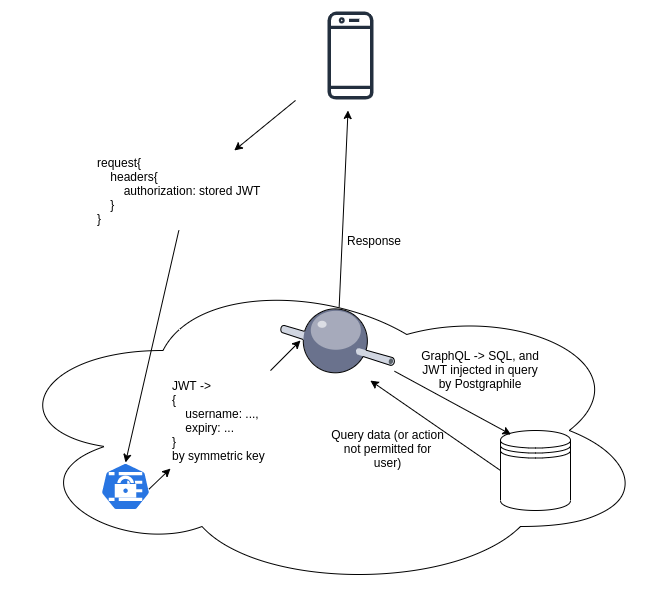
\includegraphics[width=1.0\linewidth]{authentication.png}    
    \caption{
  Once the user has stored the JWT token, this is how authentication works
    }
\end{figure}


\subsubsection{Authorization}
Now that the database can authenticate users, it still needs to check whether a particular user has rights to perform an operation. This is implemented through row level security policies. Row level security policies only allow operations if the affected row(s) evaluate to true for the supplied boolean expression.

This following row level policy only allows a user to send a message as themselves in to a group that they belong in. These rules can also be written for selecting, updating and deleting. Although verbose, this creates consistent rules that are written once and enforced by default everywhere. This prevents bugs that cause data leaks (for instance, you can't accidentally send a group another group's chat messages, as this wouldn't be permitted by the RLS policies).

\begin{lstlisting}[language=SQL, caption={Row level security policy only allowing a user send messages as themselves to their team}, ]
CREATE POLICY chat_message_create ON "chat_message" FOR insert to query_sender with check (username = (select username from active_user()) and groupName = (select groupName from active_user()));
\end{lstlisting}

\subsubsection{Password Management}
When a user creates an account by sending an encrypted POST request, I hash and salt the password and store the username in plain text.

\begin{lstlisting}[language=SQL, caption={Hashing and salting done with pgcrypto}]
insert into "user"(username, password) values (username, crypt(password, gen_salt('bf')));
\end{lstlisting}

Then, when a user requests a JWT token, I simply hash their input password again, and compare it to the stored one:
\begin{lstlisting}[language=SQL, caption={Hashing and salting done with pgcrypto}]
if authenticated_user.password = crypt(input_password, authenticated_user.password) then
  #grant JWT
  #...
\end{lstlisting}

\subsection{Business Logic on the Database}
With the current setup, we can execute simple authorized rule-based CRUD operations. Usually we want more complex logic. One solution would be to replace the automatically generated queries and mutations with custom ones which also include side effects. This would go against Postgraphile's philosophy of reducing the amount of source code that needs to be written. The best way to introduce side effects was to use database triggers. Database triggers are functions that execute when specified events occur. Triggers can alter the row that caused the trigger to execute, as well as execute SQL that impacts other rows/tables.

\begin{lstlisting}[language=SQL, caption={Definition of a function which sets the row's ``updated\_at'' column to be the current time, along with a trigger which binds it to user updates.}]
CREATE OR REPLACE FUNCTION trigger_set_timestamp()
RETURNS TRIGGER AS $\dollar$$\dollar$ 
BEGIN
  NEW.updated_at = NOW();
  RETURN NEW;
END;
$\dollar$$\dollar$ LANGUAGE plpgsql;

CREATE TRIGGER set_timestamp
BEFORE UPDATE ON "user"
FOR EACH ROW
EXECUTE PROCEDURE trigger_set_timestamp();
\end{lstlisting}

Triggers require less code than implementing a function from scratch, as I only need to define what happens after a read/write (handled by Postgraphile). They also reduce the amount of code which needs to be written in other places. If I had two functions which both updated a user, the updated\_at timestamp would be updated automatically from both. Without a trigger, you need to update the timestamps in both functions separately. I found that I needed to be careful when implementing triggers, as triggers can cause other triggers to execute. This makes the code difficult to debug, but is also potentially dangerous as it can lead to infinite loops (leading to big AWS bills). A good rule of thumb was to avoid executing triggers through other triggers.

\subsection{Implementing Real Time Client Events}
In order to make real time social interaction possible, I set up a live event feed of user workouts, personal bests and user messages. In order to implement real time events on the server side, I used Postgraphile's built-in websocket subscriptions. Client subscribers listen to a ``topic'' which is a string representing a real time event source. A topic ``blog\_posts'' might notify listeners with a link to the new post whenever a new blog was published. In my case, I had topics for every team, which were formatted as ``Event\_{Team Name}'' (such as ``Event\_Dream Team''). Postgres alerts Postgraphile when a user event has been inserted in to the database, along with the name of the table and ID of the row (such as new workout with ID 24). Postgraphile forwards this information to all subscribers through the websocket connection. The client is responsible for presenting the different events. 

\subsection{Deploying Server and Database}
I originally intended to deploy both my database and server on Heroku, as I was familiar with both. I realized that Heroku's database wouldn't fit my use case: you are not allowed to create roles. My security policy is built on having a super user (which only I have access to) and a restricted regular user subject to all security rules. Postgraphile is connected as this restricted user, so any GraphQL (and thus SQL) that a user sends is subject to row level security policies. With only one superuser role, all SQL that Postgraphile forwards would be as the superuser, which would nullify all security rules. I considered hosting the database and server on AWS, but Postgraphile does not support subscriptions there (due to the serverless infrastructure). I decided to combine the best of both worlds, and used a Heroku server alongside an AWS RDS database (which supports roles, even on the free tier.) It took some work for me to get SSL properly working as I am new to using AWS. Locally, simple queries took 10-20ms, whilst more complicated queries involving triggers took 50ms. With my current hosting, this was about 100ms for simple queries and 200ms for complex ones. I was very pleased with this, especially since I was using free tier on both Heroku and AWS. 

\subsection{Implementing Relative Strength Calculations} \label{strength_calculations}
A key part of my app is the connection between in game strength and real life strength. Strength is hard to calculate, as it depends on factors such as the exercise, the weight used, number of repetitions, the bodyweight of the user, etc. Although formulas exist for popular exercises (such as squat, bench, and deadlift in powerlifting) I wanted the app to include more exercises, especially bodyweight ones during COVID-19. I did some research, and couldn't find any APIs that handled these calculations, but I did find websites. I contacted the owners of the sites, and they weren't willing to provide API access. Luckily, the owner of Strength Level didn't mind me scraping their site. Strength Level's web client contacts an API to make these calculations, and by tracking my network requests when I submitted the form, I could copy and analyze how my request parameters were sent. The form submission request sent HTML responses which I could scrape to extract the percentage. You can see the form as well as the HTML it returns in Figure \ref{fig:strength_level}.

\begin{figure}[H]
    \begin{subfigure}[t]{0.45\textwidth}
        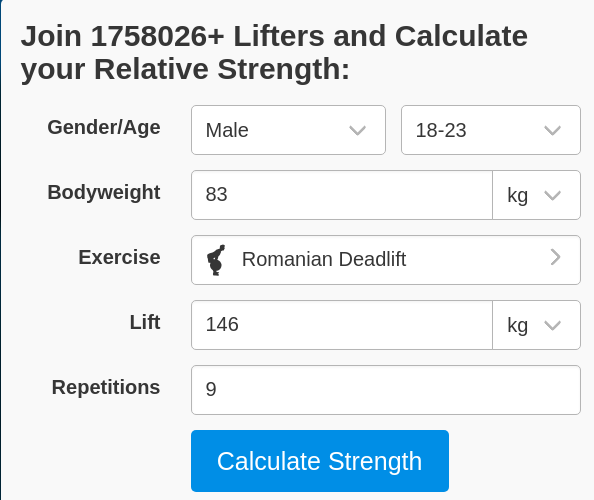
\includegraphics[width=1.0\linewidth]{strength_level_layout.png}
        \caption{Strength Level's form which I submit automatically from my server} 
    \end{subfigure}
    \begin{subfigure}[t]{0.45\textwidth}
      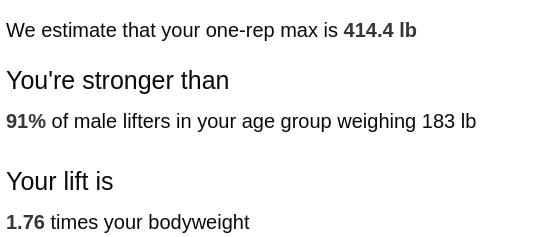
\includegraphics[width=1.0\linewidth]{strength_level_stronger_than.png}    
      \caption{The HTML which this form submission returns, which I use to extract the "stronger than \%" value}
    \end{subfigure}
    \caption{Strength Level's layout}
    \label{fig:strength_level}
\end{figure}



I then made the exercise request generalizable (for instance, by changing the exercise which I submitted, ``romanian-deadlift'') to the variable exerciseName. The node.js server didn't allow for the Strength Level request to be made, as it wasn't encrypted. After doing some research, I found two solutions: one would be to disable this restriction and to send the request without any encryption. This is a bad idea, as the request contains some sensitive information (exercise performance, identified gender, weight). This would also remove warnings when sending unencrypted requests to other hosts. The latter solution involved getting the public key (.pem file) of Strength Level, and encrypting the request with it. This was harder, as I didn't have experience with this, but I'm glad I learned to do it properly (as I also needed to configure Amazon's public key for database requests).

Most of the request parameters were self-explanatory (exercise weight, bodyweight, repetitions, etc.) as it was obvious that they were just numbers. The exercise name parameter required more work to generalize, as this was a string which had to be in the small subset of Strength Level's supported exercises. I scraped the names by copying the HTML of the exercise browser, and by stripping everything but the names. This was initially enough information to set up relative strength calculations. Months later as I tracked a bodyweight exercise, I found that the request didn't work. This is because bodyweight exercise have a different request format. Instead of requiring lifted weight as a parameter, they require ``additional\_weight'' and ``is\_bodyweight''. To accommodate for this, I added an extra database field to all my exercises (is\_bodyweight), scraped all exercises tagged as such, and set is\_bodyweight to true for all those exercises. The request format also had to change depending on if the exercise was bodyweight or not. After fixing this bug, it was very easy to add a ``bodyweight only'' filter to the exercise search in my app, which hopefully let some quarantined users participate. 

I accidentally mislabeled two exercises as bodyweight, which lead to one user's client repeatedly crashing. My server threw an error, as Strength Level didn't give a valid response from the malformed request, which gave the user an error as well. The client would try to resend it whenever they relaunced the app, which led to more crashes. I fixed these exercises in the database, and told the user to remove their cache (which stopped the user from trying to send a malformed request).


\section{Client}
\subsection{App Technology}
As I already had some experience with React, I decided to use Expo, which is a superset of React Native. There are some differences, mainly that components use different tags (a basic container is called a View as opposed to a div). I quickly realized that React Native isn't simply about developing one code base. When installing some libraries, you would need to configure the Android Kotlin code, or the Swift code of the iOS app. I was intimidated by this, as I had experience with neither language or build system. Another issue is that I was developing on Linux: testing and building the iOS app was difficult, so I wanted the iOS app to stray from the Android version as little as possible.

Expo is slightly different from React Native. You can create a React Native app through Expo without touching a line of platform specific code, unlike in React Native. Expo also handles certificates and keys for you, which was enticing, as I didn't even know what they were. It is also easy to convert back to React Native if I wanted to. 

\subsection{Expo App Size and Launch Time}
React Native apps compile into platform specific classes and components, e.g. a React Native <View/> component becomes a Swift UIView on iOS, and a Java/Kotlin View on Android. Any Javascript that you write, or Javascript libraries that you use will stay as Javascript which is a slow language. It is not compiled like native app languages, and instead interpreted. This could prevent some older devices that already have performance issues from using my app. In my case, the app was reasonably simple, and much of the data processing was handled server side, so this was not much of an issue. 

\citet{app_size} compared the sizes of different APKs generated by Java and React Native. A simple app that showed ``Hello world'' to the user 539 KB, while the React Native app was 7 MB. This is primarily caused by the bundled Javascript interpreter which the React Native app bundles along with the App. This is not a requirement for Java apps, as Android devices already have a Java Runtime Environment. App size only gets worse with Expo: ``An application with Hello World weighs 25 MB'' \citep{expo}. App install size is very important: ``For every 6 MB increase to an APK’s size, we see a decrease in the install conversion rate of 1\%'' \citep{app_conversions}. This article primarily stresses the importance of app size when developing apps for countries with poor network connectivity and cheaper devices. My participants primarily resided in Finland and United Kingdom, where storage and network connectivity weren't as much of an issue. None of my participants reported that they couldn't install the app. There is also a difference with download and install size: The Android App Bundle (aab) is about half the size of an APK to download, and this bundle is also compressed. My app download size was about a fourth of the installed size.

One of my primary concerns was the startup time of my app. A device must first load the 'javascript bundle' into memory, which is a file containing all the Javascript of the app. This is usually unnecessary, as an app has multiple screens and sections which are only required when these screens are opened. With this default behaviour, my app took 5 seconds to open. This gives bad first impressions, and might make some users think that the app has crashed. Slower startup times would also increase the barrier of entry for tracking workouts and engaging with your team, which would reduce app use.

In order to alleviate this, React Native allows you to load the bundle dynamically in chunks as they are needed. This also reduces the load on the server: components which send requests only do so when this request data is shown to the user. Every modal and overlay is only loaded into memory when it is opened and the group tab is only loaded once the user has navigated to that tab. One of the most important lazy imports that I implemented was for the app and the app demo. The app demo is only needed if the user hasn't signed in. Conversely, the app is only needed after the user has gone past the app demo and signed up. One issue with this implementation is that we need to receive a server response validating that we are signed in and that our JWT token hasn't expired before we can decide whether to show the app demo or the app itself.

Luckily my query client, Apollo, has a solution for this. You can configure Apollo to cache queries in the devices' local storage. When executing a query, Apollo initially shows the data that the server responded with last time. Once the server sends an updated response, Apollo presents the server data instead. When the local storage of the device matches the server, the query is unnoticeable as there is no change from the client's perspective. When the data is out of sync, you briefly see outdated data before seeing new, refreshed data. In the aforementioned login case, our app assumes that the user's login status has not changed since last time and loads just the previously used screen. If the user was signed out, they would be taken back to the login after briefly seeing their last used screen. If the local login state matches the server state, the user does not even notice that I checked their sign-in status. I use caching for most of my other queries as it doesn't require me to compromise between staying synced with the server and making the user wait. There were some cases where this caching policy led to accidental features. When you open your team tab to view the state of your monster, you initially see the monster sprite and the health when you last viewed it, before the health/monster updates (if other users worked out while you were gone). This shows the user of the progress that was made while they were gone.

Apollo's cache also leverages Postgraphile's ``globally unique identifier'' implementation. This concept was introduced by another query client, Relay. A globally unique identifier is an identifier which is not only unique for a particular type, but for all types. For instance, a user and a group cannot have the same globally unique identifier, even if some have the same primary keys. Postgraphile implements this by sending a base64 encoded string containing the name of the type, along with the primary key of the type, which is unique for all rows for all tables. This allows Apollo to merge and cache data more efficiently, and to refetch data more sparingly, without requiring me to specify the primary keys of every single table.

\subsection{Development Technologies}
I used Typescript during development of the app, which is a superset of Javascript containing type checking. Typescript is not shipped with the app: it is compiled into Javascript. Javascript was designed to absorb errors in production, which is good, as a slightly malfunctioning app is usually better than a crashed one. Typescript enforces what Javascript does not enforce in development, such as null checks, supplying required parameters, and more. All parameters supplied to React components are optional in Javascript, which can lead to errors being thrown by the child component, but not in the parent which neglected to supply a required parameter. Typescript also enforces the types of the parameters, which prevents weird type issues which Javascript is often known for.

%MAYBE
\subsection{User Path Tracking}
I set up simple analytics tracking to better understand how the client was being used. Whenever a user opens an overlay or navigates to a screen, it sets a global visibleSection variable to its own name. I set up a listener for this global variable, which appends the section value to the end of a list whenever it changes, along with the time that was spent on it. This results in a timestamped sequence of user actions  This listener sends this user session path to my server when the user closes the app. When the analytics are sent, the path is set back to an empty list to avoid sending the same path twice.

\subsection{Player and Enemy Sprites}
In order to make the app more lively, I bought an animated pixel art sprite pack from an artist. I ended up using 6 different characters, and 8 different enemies. The sprites had varying amounts of whitespace padding around each frame. Fights would look weird with the enemy, as they wouldn't be centered vertically. I tried to solve this by applying absolute positioning to the characters, but this would break depending on the device. Eventually, I removed the whitespace from the sprites manually through a bash script using ImageMagick, a command line image editing tool. Each frame of the sprite sheet needed to stay the same size. My script required the number of rows and columns in the sprite sheet in order to calculate the size of each frame, as well as the percentage that should be clipped from the top, left, right, and bottom of each frame. This was a bit tedious but it worked.

In order to make the characters idle, I simply had to loop the idle sprites. Battles were a bit more difficult to implement. I triggered the player attack animation, which had an onFinish() function hook. The player's onFinish() call triggered the enemy ``on hit'' animation. The onFinish() call of the enemy triggered the player to attack again. This repeats until the enemy is dead, the player has no more attacks, or the player skips the animations.

The client stores the sprites on the device, but the server tells the client which sprites to renders. Sprites are loaded into memory lazily only once they are needed.

\subsection{Deploying to App Distribution Platforms}
Deploying the app to Google Play was very easy. I had done all of my development with an Android device, so I didn't need to do extra testing, and my first production build was accepted. For iOS, it took a few days to make sure that everything was working as expected. I primarily had to make sure that text sizes and buttons were well sized for Apples flagship phones, and that safe area views were working properly. I also had to take screenshots with multiple devices, create a privacy policy, and do just about everything I did for Google Play again. My app was rejected 5 times over a month before it was finally accepted. This was primarily due to Apple's new strict policies on health studies.

\chapter{Evaluation}
In my evaluation my primary focus was users' view of team and user progression. My hybrid model can be considered effective if some users weren't interested in one goal, but they were interested in the other. These users would have dropped out if the app only supported the one goal they didn't care about. The model can also be considered successful if the personal goal augments the shared goal for some users, or vice versa. The multiple goals have the drawback of making the game more complicated: the model can be considered unsuccessful if more users were confused than helped by it. 

I conducted interviews in a semi-structured fashion, which let me explore emerging themes.  

\section{Participants}
I had a total of 24 participants Participants were recruited through messaging apps. I only directly contacted friends. Some people invited their friends who I did not know. My app required users to sign the consent/participant information form before signing up and using it, so I did not need to provide much information to the user initially. All users were asked to participate in a survey. I asked users to forward the survey to any of the friends they invited. Through diversity sampling based on analytics data, group membership and activity levels, I invited 10 users for an additional interview. The mean age of participants was 22.8 and 93.3\% identified as male, the rest identifying as female. 53\% were in the UK, 26\% in Finland, 13\% in America, with the remaining 8\% from the Czech Republic. 

After looking at the survey data, I realized that my study recruitment had a strong sampling bias. I wanted to share my app with people who would fully understood and appreciated it, such as experienced lifters or users with gaming experience. For instance, 86.7\% of users had performed some kind of strength training in their lives. Every user had regularly performed some form of exercise. These users mostly had lots of experience, as you can see in Figure \ref{fig:long_performed}.
\begin{figure}[H]
    \centering
    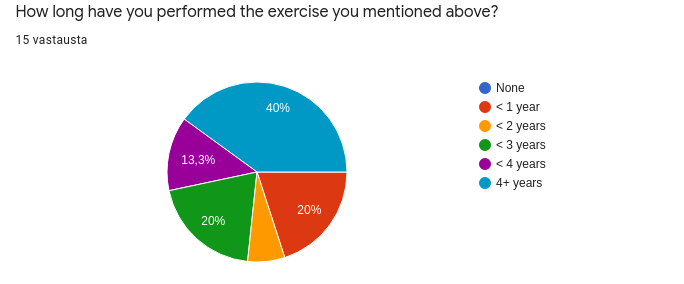
\includegraphics[width=1.0\linewidth]{long_performed.png}    
    \caption{User exercise experience}
    \label{fig:long_performed} 
\end{figure}
%6.0 What you hope to gain, quantitative results, 6.4 qualitative results, 6.5 thematic analysis, 6.6 summary of evaluation

I tried to address this in the interview stage by sampling users who didn't use the app much, and those who did not have much training experience. 


\section{Methodology}
My surveys mostly collected quantitative data. I thought it would make the most sense to ask more qualitative questions in interviews where users could go into more detail, and I could guide discussions. The survey asked for some demographic information (age, identified gender, location) and questions related to my research. I conducted my interviews semi-structured: I would prepare questions which where specific to that user. For instance, if I sampled a user because they were the most active in their team, I would ask what motivated them, how they viewed their lower performing teammates, etc. Once I had answers for the user-specific questions, I would let the user speak freely, interrupting as little as possible. This helped me discover known unknowns, leading me to discover issues and ideas I wouldn't have found in a very structured interview. I transcribed all interviews with otter.ai, an audio transcription service. I went over each transcription, noting their responses to my prepared questions, as well as any other issues which the user raised during the unstructured part of the interview. Once I had condensed notes of each participant, I performed thematic analysis to identify emergent themes along with evidence. 

\section{Survey Data}
In Figure \ref{fig:intensity}, you can see the ratio of users who claimed that their intensity increased when using my app. This app seems to have motivated some users, but not a very meaningful share. I also forgot to include an option for users who exercised less while using my app, which has been grouped together with "did not exercise more". Many experienced users had rigid plans which they didn't want to stray away from. For instance, User 4 commented: "This app was motivating, but I paid for a plan with exact sets and RPEs, so I didn't change my training". This question should have asked about motivation, and not the actual physical workout intensity.
\begin{figure}[H]
    \centering
    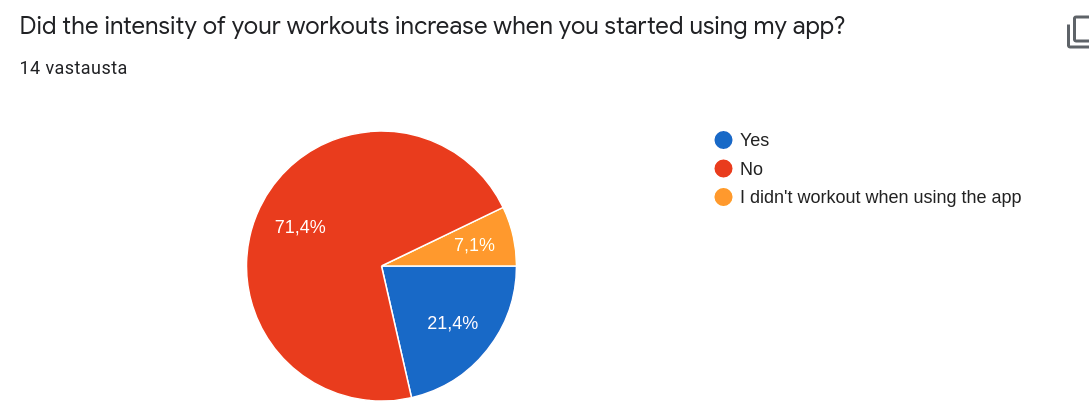
\includegraphics[width=1.0\linewidth]{exercise_intensity.png}    
    \caption{Self reported change in exercise intensity}
    \label{fig:intensity} 
\end{figure}

I asked users how often they trained prior and while using my app. The results are visible in Figure \ref{fig:workout_frequencies}. The mean workout frequency is slightly lower while using my app (4.2 vs 4.13 workouts/week). There seems to be a simultaneous increase and decrease in exercise frequency. One user who exercised four times a week removed a weekly workout, whilst another user added a fifth one. This data suffers from the same issues as Figure \ref{fig:intensity}, as many users have rigid plans which they don't want to change. The difference in mean, as well as the size of my sample are very small, so no conclusions can be drawn from this.
\begin{figure}[H]
    \centering
    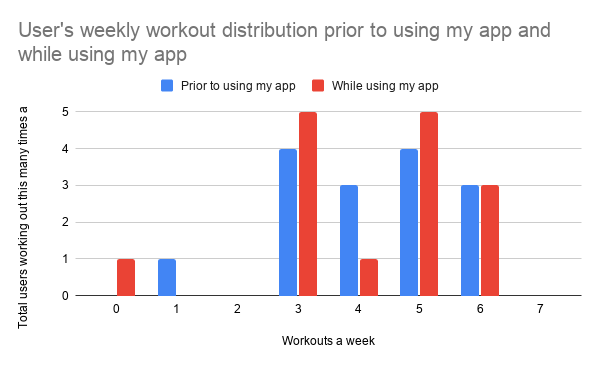
\includegraphics[width=1.0\linewidth]{user_workout_distribution.png}    
    \caption{Frequency prior to using my app}
    \label{fig:workout_frequencies} 
\end{figure}

Finally, I asked users how motivated they were about progressing their team and their character, the results which are in Figure \ref{fig:character_vs_team}. The mean interest towards both was very similar (3.4 for character, 3.2 for team). Interest in developing character seemed to be much more stable than interest in developing the team (4/5 for 66\%). This means that personal motivation can serve as a fairly reliable fallback for those who do not care about helping their team. 
\begin{figure}[H]
    \centering
    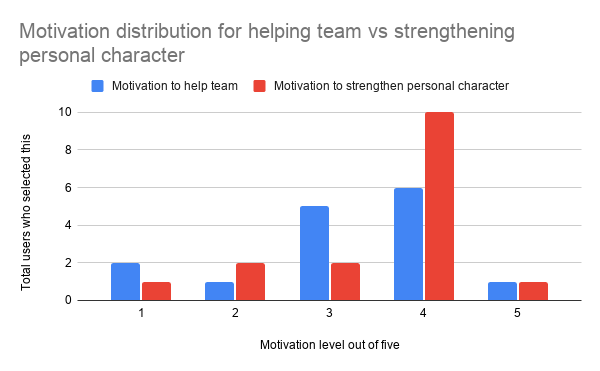
\includegraphics[width=1.0\linewidth]{moviation_distribution_team_character.png}    
    \caption{User motivation to improve their character vs their team}
    \label{fig:character_vs_team} 
\end{figure}




\section{Interview Thematic Analysis}
\subsection{Shared vs Personal Goals}
Users had more mixed views towards shared goals over personal goals. This confirms that the personal goal can serve as a much more consistent fallback for the group goal, as we saw in Figure \ref{fig:character_vs_team}. There was one user (User 2) who treated the app as a personal tracker but did not join a team: ``I've seen kind of similarish ideas before. Like habit tracker apps that are kind of like RPG, where you can develop your own character. So I kind of viewed it like that. So it's kind just personal motivation for you.''  User 10 mentioned in addition to not having access to the gym: ``For me working out is a personal hobby and I'm not interested in making it group-based''. User 6 had a similar response ``In RPGs you grind and train alone, and you taking that experience away is weird.''. 

There were two users who didn't engage with the personal goals of the app, but were a part of the group goal. User 1 called these users "moral support". They never contributed to the goal, but they warned the team when the enemy was about to expire, and welcomed new users who joined the team. These users did not engage with the personal goal, and having a shared goal still allowed these users a different way to play the game. Although this did not increase exercise for these users, User 1 still liked having them there: "they're kind of like an audience". 

\subsection{Reaction Towards RPG Features}
Users liked when gym and RPG references were combined. Users enjoyed creative names like Frogman, King of Deadlift Leverages over generic monster names like ``Mudcrab'' and ``Minotaur''. User 1 said: ``I mean, it's funnier to do frogman jokes. Like deadlift guy than frostcave guardian and stuff like that, which is not like related to gym''. This particular ``Frogman'' character evoked strong reactions from many user. When aforementioned User 1 killed the Frogman character, they sent a message: "Get the **** out of here Sammakomies" (Sammakomies is Frogman in Finnish). Another user from another team had a similar reaction to the Frogman character. User 7 announced a workout they planned for the next day with: ``Frogman bouta get slapped the **** up tomorrow''. After User 7 completed the workout, another user in the team, User 8 commented: ``Yo frog man got ****** up'' and ``0 ROM deadlift looking ***''.  You can see a frame of the Frogman's sprite sheet animation in Figure \ref{fig:frogman}. This character successfully increased social relatedness through the users having to overcome a common enemy, as well as drove positive interaction through humor, like I intended in Section \ref{enhancing}. In both teams in which someone mentioned this character, one or more users also started talking about him.

User 7 mentioned how he enjoyed tracking workouts as he could see the enemy take damage in a battle ``Oh, you know, I get to put in, 14 sets or whatever I did. And I get to see the boss taking damage.'' User 4 also mentioned the satisfaction of entering workouts: ``I kind of saw it as a sort of a motivation thing, and sort of to get you to train and give you the extra wee bit of dopamine from training and when logging your workout''

Generally, users suggested adding more sounds and animations. User 6 suggested that all inputs should have some kind of satisfying feedback: ``If it's not visually stimulating it's not going to be interesting, it's like filling out a spreadsheet''. User 7 used the term ``dopamine factory'' to describe making the app as addicting as possible. This would involve animations and sounds, and adding a ``lootcrate'' system to the game, where users unlock chests containing items, which would all be animated. 

A common feature suggestion was that exercises should be divided by body part. In addition to making searching for exercises a bit easier, users suggested adding this as an in-game feature. ``Yeah it makes kind of sense if you have body part specific armor that maybe if you do arms a lot you get a battleaxe.'' Other users suggested different ways converting real world to fantasy, such as different character builds based on your strengths (if you're good at cardio, you might be an agile character). Some users suggested making RPG style quests: ``If you kill a certain enemy 10 times you get a weapon''. These quests could also be connected to the real world: ``do squats 2 days in a row for extra gold''. Although unrealistic, one user suggested giving sponsored prices for in-game achievements: ``First person to reach x level or beat y challenge wins something such as supplements from a sponsor''.

Although most users agreed that real life strength should remain important, many suggested adding rewards which are based around using the app: ``There should be rewards for using and engaging with the app that don't require real world improvement''. Rewarding app use would hopefully reduce inequalities amongst beginners and users which already train.  User 7 and User 8 had a beginner in their team who tracked only one workout, but dealt a fraction of what User 7 and User 8 and lost interest. Small inequalities can be motivating: for instance, User 8 worked harder to catch up to User 7. When this gap gets too big, users lose motivation. There are many 'pay to win' apps which let users play the game for free, but which lock long-term progression behind a paywall. I could copy this, but through a 'train to win' model, which would only allow users to progress beyond the early stages if they train. 

A couple users did not like how I had implemented overflow effects. By default, any damage that brings an enemy below zero health is wasted, and not dealt toward the next enemy. This was easier to implement, and I decided to leave it in to see if this would lead to more collaboration. Users would need to coordinate their workouts amongst themselves to minimize wasted damage. Nobody viewed this as something to collaborate together on, but rather as a technical problem which should be addressed.

\subsection{App Design Comprehension}
Experienced users seemed to understand how the app worked. For instance, one of the strongest users ``liked the simplicity of the app''. This was not the case for beginners. User 6 thought ``it was a bit scary and disorienting to start using the app''. Experienced users only had to understand the game side of my app, but beginners had to understand the exercise aspects as well as the game aspects. I discussed how I could better implement tutorials with users who didn't understand the game. No user seemed to care about the pre sign-up tutorials. Users that skipped the initial tutorials said they would have been more receptive to embedded tutorials, such as an explanation of a section as you open it. Some users suggested some fun ideas: such as making an animated pixel art guide, in-line with the games' theme.

I tried to identify what made the app difficult to understand. Users who did not understand the app at all couldn't point to the specific thing which they found confusing, as they understood none of it. I have reason to believe that on average strength tracking was more confusing than the RPG model. I had many users who played games without training experience who didn't understand how the app worked. For instance, User 5 was an avid World of Warcraft player who had also played mobile RPGs such as Clash of Clans. He was able to join a team with a friend, and understood the concept of personal progression. He never tracked any exercises, as my app didn't give any sample workouts, or contain any exercise guides. On the other hand, quite a few users had never played RPG games, but were still able to participate in the game. User 9 had training experience, but had never played an RPG game. She understood the concept of developing her character and helping the team. But even she was confused by the exercise tracking: she thought that the personal bests screen was the workout tracking functionality. As she was exercising, she would update the personal best for the same exercise multiple times, even if her record reduced. 

The exercise concepts of the app could be introduced separately from game concepts. For example, users could first be given armor and weapons that they could equip and use, but some items could only be equipped after submitting personal bests. Beginners would be able to comprehend the game and play it, but wouldn't feel pressured to understand the exercise side unless they wanted to progress faster. 


\subsection{The Strongest Members of Teams}
User 1 and User 3 were users that contributed a substantial amount of the damage to the team (80\%+). Both the users had a lot of training experience. User 3 was the strongest out of all users, and User 1 was above average in strength, and had used an activity tracker named ``FitNotes'' before. I was interested in what drove them to contribute such a large amount, and how they felt about doing so. 

Both of these users mentioned competitiveness, but hardly anything about collaboration. It is hard to say whether competitiveness drove these users to perform better, or if they became competitive due to their superiority. For instance, User 1 wanted more transparency towards other members' actions, so that he could compete better: ``you could click it and see all the movements that they did in the gym, the weights and the reps. I think it would be a bit more interesting. And for people who like competition it would be fun.''. User 3 thought that being able to see the damage and actions of other users leads to competitiveness and more actions ``Oh, ****, User 3 is out there, I've got to do the same''. 

User 1 and User 3 had very opposite reactions towards being the best in their team. User 1 commented: ``If everyone would have been contributing equally, I think I would've put much more effort into it.'' At one point, User 1 had sent a chat message asking if the other members had gym access. He later explained that this was a passive aggressive way of asking why the other users weren't contributing enough. 

User 3 reflected on his gameplay with ``Plus, I was carrying those noobs'' in a satisfied tone (``carrying'' in games refers to single-handedly winning games for your team, and ``noobs'' are beginners). Although he clearly enjoyed being the best in his team, he didn't think it would be fun if someone else was outdoing him by a large margin: ``And then we had one guy who was working out seven out of seven times a week for three to four hours a day. And so imagine that we had that guy in our team: he would be doing like 89\% out of a team of 10 people.'' 

Both users suggested fixes to balance the user contributions. User 1 suggested that the game should rely on each team member more, by dividing users into different classes with different responsibilities. ``You will even have a kind of social pressure to do a workout. If your team's success is based on your stamina stat or something like that.'' I had considered increasing per-user responsibility more. I decided not to do this, as I didn't want to inactive users to prevent progress, but only to slow it down. I asked this user how they would feel if they had to rely on someone who was not active. User 1 responded: ``If my progress in the game would be relying on someone who doesn't do anything. I think it would be a bit unmotivating for me.'' 

User 3 had a suggestion that involved changing how the game behaved, rather than how user actions should be influenced. He suggested adding ``bonus damage, which might be the adjusted percentage of the monster's health. So it doesn't matter how weak you are, you could still offer the team that percentage damage''. This would mean that everyone's effort would be equally valuable. Users would still contribute more to their team through being stronger, but this would allow weak users to contribute equal amounts in at least one dimension. 

In another collaborative activity tracker, Pass the Ball, a similar issue arose in the first trial of the app: "they realised that the best strategy for them in game terms was to let the most active person in the team (who worked as a bicycle messenger) keep the ball indefinitely." \citep{Pass_the_ball}. My pilot study only had two users who had similar activity levels. A larger pilot study with a larger diversity of users would've exposed this design flaw.

\subsection{Team's composed of strangers}
I prevented the formation of 1-person teams as these users wouldn't be collaborating with anyone. I didn't want users to drop out if they didn't want to invite anyone, so I added a ``Join Random Team'' button, which would place you in the smallest and oldest public team. This led to teams with 2-3 members forming, where users did not know each other. I was curious of how these teams performed compared to teams where users knew each others.

Much like research by \citet{Fish'n'Steps} found, anonymous teams did not perform well. User 2 tried to create their own team, but wasn't allowed to play without other members. They didn't want to invite their friends to play, and realized that their only option was to join a team with strangers. User 2 didn't want to do this: ``So I thought it's kind of weird just joining a random group, that I don't know the people in.'' 

Although User 3 was reasonably active, he thought his experience could have been better: ``If it was under normal circumstances, and I would actually have my friends and not just strangers, it would be really fun.'' 

User 4 didn't feel negatively about working with strangers, but didn't care about their team: ``It was almost like I was doing it myself because I didn't know the guy'' 

The sentiment was also reflected in the activity levels of the users. The two most active teams were composed of users who all knew each other.

\subsection{Altruism vs Obligation}
I asked members who actively contributed to their team whether their motivation to help was altruistic or due to social obligation. Altruism can be viewed as a positive motivator, wherein users view their contribution as a voluntary gift to their team. Social obligation is a more negative motivator which makes uses feel that they have some responsibility towards their team, or they might be viewed poorly. Users seemed to be unsure about what drove them to contribute to their team. User 8 responded: "Good question, I'm not really sure. I guess it was about helping the team but also not being viewed as lazy." As I implemented techniques from social support theory and social comparison theory, users seemed to be motivated by both altruism and obligation simultaneously.

\subsection{Collaboration vs Competitiveness}
User 7 and User 8 were both in the same team. I asked both users individually whether their motivation was driven by collaboration or competition. User 7, who was strongest in the team responded: ``I think, at the start, I would tell User 8 'Yo, I just did a workout I just did this much damage, the boss is almost dead, you need to work out'''. This was mostly collaborative: User 7 trained to help the team out, and wanted the User 8 to help him defeat the enemies. I asked User 8, who was a bit weaker than User 7 the same question. He reiterated the same sentiment as User 7: ``We never spoke about being competitive''. He confessed that he felt competitive, although he didn't express it: ``I think User 7 did a couple more workouts than me, and I was trying to keep up with him. I think it was definitely competitive there.'' This intrigued me, as User 8 felt competitive as the underdog, but the strongest member in the team did not. It also led to User 8 putting in more effort: ``The app probably added an extra workout every week''. This is what I hoped that the app design would lead to: users that are weaker and who train less wanting to keep up with other users.

\subsection{COVID-19}
Almost all interview participants mentioned COVID-19 at some point, generally as a reason for dropping out or not starting. There was a strong correlation with gyms access and training activity. I had 4 different people from Finland, which was the only country from which participants had gym access throughout the study. All 4 joined teams and tracked workouts. The most active team had 3 people from Finland.

User 10, who resided in Scotland shared why they didn't start using the app. ``Gym access is like the first issue, obviously, because that was my primary source of exercise. Like, I'm literally just not doing anything''.

User 3 performed bodyweight exercise despite gyms being shutdown. He couldn't get any friends to use it, since none of them had gym access, and didn't bother bodyweight training: ``Timing was kind of bad because nobody I know was working out during the three weeks I had to actually test it. Even in other countries, they were in countries that are currently locked down. So they couldn't go to the gym. I'm still working out. But that's because I do bodyweight stuff, so I can do it''

\subsection{Ethical Considerations}
I implemented alerts which were triggered if users progressed too quickly in order to prevent users from progressing without caring about technique. Users raised other potential ethical considerations about my app which I had not accounted for. User 1 mentioned how my app could lead to users doing too many workouts: ``If I do like five gym sessions per week, but if that wouldn't be enough [to defeat the enemy], it wouldn't be very good for my health like to do like, seventh or eighth, gym session.''. In a similar vain, User 4 thinks that my app could lead to users prioritizing game progress over sensible training if the game is poorly balanced: ``You shouldn't be able to game the system, do lots of fluff work just to inflate your numbers, all training styles should be accounted for''. User 7 mentioned that I should be considerate about adding new features, such as calorie tracking: ``It would probably lead to eating disorders where people lose a bunch of weight''.


\subsection{Commonly Mentioned Technical Issues}
By far the most mentioned issue was a keyboard opening error. If you searched for exercises and tried to set the repetitions/weight of the last or second last element of the list, the keyboard would overlap with the input, which would close the keyboard as soon as it opened. Users could luckily work around this: as long as they specified their search more, the last element would appear as the first element, which allowed the user to input the values.

Another commonly mentioned issue that was mentioned was the compression of the splash screen. I was aware of it but didn't have time to fix it. 
One almost game breaking feature was that the keyboard would almost block the ``track workout'' button on larger iOS devices. I had more bugs on iOS, as I did most of my testing and development on an Android emulator.

There was an interesting bug with number inputs. Any number inputs (such as weight lifted) would open a numeric keyboard. I suppressed Typescript's warnings about parsing the input strings as an integer or float, as I thought user's wouldn't be able to enter non-numeric values. If users pressed backspace when the input was empty, my app would parse the ``backspace'' string as numeric, which caused a crash. This also wasn't game-breaking: users just had to be careful to not press backspace more than necessary.

This bug was only visual, but the fight with the players character and the enemy was off center and sometimes slightly off-screen. The bug could have been avoided by using a larger array of emulators with a diverse number of screen sizes. This lack of device test coverage led to other similar bugs. Although I had implemented flex views which scaled proportionally with screen size, elements such as buttons and text did not, which led to small elements on some screens. Users with larger screens sometimes didn't even notice the ``User'' and ``Group'' labels on the bottom navigations tabs, which is an important part of the app.

\section{Analytics Data}
I tried to identify whether having multiple goals made the app more confusing to use. In order to identify this, I looked at the user paths of users who didn't understand how the app worked. My app divided the personal goal and shared goal into different sections. The group section which contains the shared goal couldn't further confuse the user if they didn't visit it. On the other hand, if users viewed both sections and felt overwhelmed, then having multiple sections probably confused them further. I couldn't simply select any user who didn't use the app beyond sign-up. Some users, such as User 10 didn't use the app because he didn't have gym access, and not because he didn't understand the game. I decided to analyze the paths of two users who explicitly said that they were confused by the app. One user who I did not interview messaged me and told me they were confused by the app. The other user whose paths I analyzed was User 6, who said ``it was a bit scary and disorienting to start using the app'' in an interview. User paths are lists of section, time tuples. One list represent one session of use before closing the app. You can see both paths in listings \ref{lst:first_user} and \ref{lst:first_user}. Neither user ever entered the group tab. This means that they were confused by just the independent tracking, and they would have still been confused had the group tab and shared goal been removed.

\begin{lstlisting}[language=python, caption={The user paths the user who messaged me}, label=lst:first_user]
#First session
[(Set bodyweight/gender, 5.926), (View Character, 9.475), (Set bodyweight/gender, 1.286), (View Character, 5.266)]

#Second session
[(Set personal bests, 13.733), (View Character, 1.035), (Track Workout, 2.547), (View Character, 1.998)]                     

#Third session
[(View Character, 1.298)]                                                                                                    
\end{lstlisting}


\begin{lstlisting}[language=python, caption={The user paths User 6 (who was interviewed)}, label=lst:second_user]
#First session
[(View Character, 0.224)]                                                               

#Second session
[(View Character, 2.798)]                                                               

#Third Session
[(Track Workout, 2.083), (View Character, 0.974), (Set personal bests, 39.808)] 

#Fourth Session
[(View Character, 34.526), (Set personal bests, 10.047), (View Character, 3.035)]
\end{lstlisting}



I also used analytics data to analyze group size and app use. In Figure \ref{fig:exercises} you can see average number of various events from users of different sized groups. App use seemed to increase substantially as team sizes grew. There was a moderate increase in the amount of tracked exercise with team size.
\begin{figure}[H]
    \centering
    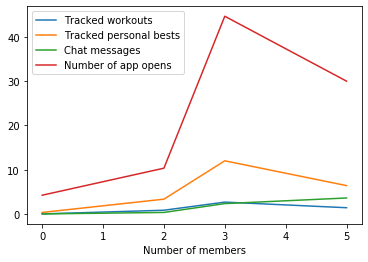
\includegraphics[width=1.0\linewidth]{data/activity.png}    
    \caption{Average number of various events for members of different sized groups}
    \label{fig:exercises} 
\end{figure}

This seems to suggest a correlation between motivation and increased team size. There seems to be no additional benefit of having more than 3 members. It is not possible to tell which causes the other: larger teams might lead to more motivation, or motivated users might join larger teams. The direction of this causal link could be investigated by placing users in teams of random size, and examining the relationship again.


\section{Evaluation Summary}
I had a total of 24 participants try out my app. These users were sent surveys, and select users were asked to participate in an interview. This app hardly changed exercise frequency, but over 20\% reported additional training intensity. There wasn't a big difference in mean interest with the shared and personal goal, but the shared interest was far more distributed. This made the personal goal a reliable fallback for those users with below average interest in the shared goal. 

Users overall seemed to understand and enjoy the RPG model of my app. The various characters which users had to fight created social relatedness, and drove positive social interaction. I tried to implement relatedness as described in self-determination theory, and positive social interaction like in social support theory. Many users thought that your in-game performance shouldn't be just determined by real world factors. Many suggested ways where users could improve in the game without any real world changes. This would also help make user contributions more equal. 

Many users seemed to struggle








%==================================================================================================================================
\chapter{Conclusion}    
I set out to create an activity tracker which had both a personal and shared goal. This app supported strength training, and gamified goals through an RPG model. 

\bibliographystyle{abbrvnat}
\bibliography{l4proj}

\chapter{Appendices}

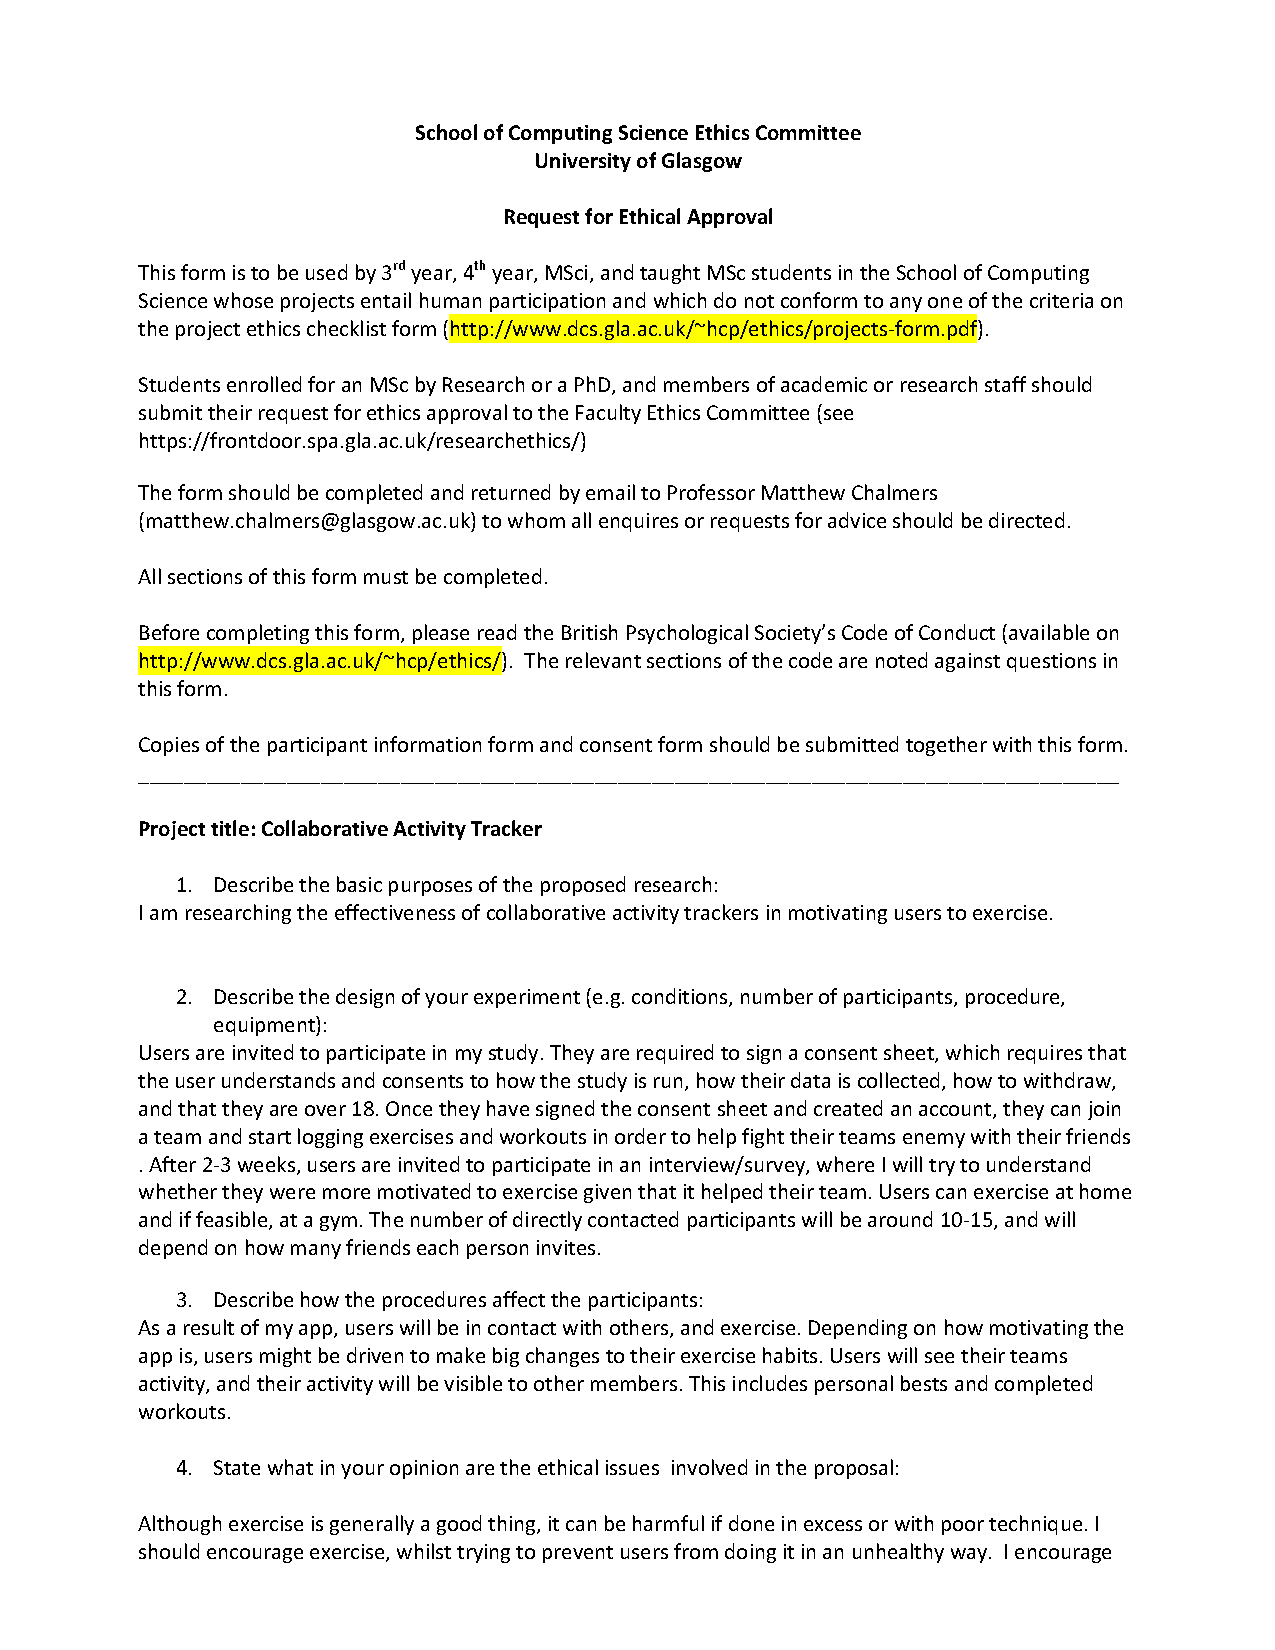
\includepdf{revised_ethics_form.pdf}
Typical inclusions in the appendices are:


\end{document}
